\documentclass[10pt,twocolumn,letterpaper]{IEEEtran}

\usepackage{cvpr}

\usepackage[utf8]{inputenc}
\usepackage[brazil]{babel}

\usepackage{times}
\usepackage{epsfig}
\usepackage{graphicx}
\usepackage{xcolor}

\usepackage{amsmath}
\usepackage{amssymb}
\usepackage{bm}

\usepackage{float}
\usepackage{multicol}

\usepackage{fancyhdr}
\setlength{\headheight}{1.5cm}

\usepackage{minted}
\usepackage{caption}

% Faz aparecer "Código" em vez de "Figura"
\captionsetup[listing]{name=Código}

% Cores do código
\definecolor{bgcolor}{rgb}{0.95,0.95,0.92}
\definecolor{commentcolor}{rgb}{0.0,0.5,0.0}
\definecolor{keywordcolor}{rgb}{0.0,0.0,0.6}
\definecolor{stringcolor}{rgb}{0.58,0.0,0.82}

% Header
\fancypagestyle{plain}{
\lhead{
\includegraphics[width=5cm,height=2cm]{logoFT.png}}
\rhead{
\includegraphics[width=5cm,height=2cm]{logoUnB.png}}
}

\renewcommand{\headrulewidth}{1pt}%


% Changing the caption and 'References' names to Portuguese.
\addto\captionsenglish{
  \renewcommand{\figurename}{Figura}
  \renewcommand{\tablename}{Tabela}
  \renewcommand{\refname}{Referências bibliográficas}
}

% to-do: Using fontenc with T1 font encoding allows \hyphenation to take words with accents
% as arguments. However, fontenc with T1 mess up with words containing 'ã' in all \subsection{}
% commands.
% If someone knows how to fix it, tell me!
%
%\usepackage[T1]{fontenc}

% Put the words not correctly hyphenated down here. Words with accents must
% be manually hyphenated in the text itself using the '\-' separator. See the examples
% throughout this template.
\hyphenation{co-e-ren-te u-sa-do de-li-mi-ta-do-res a-cer-ca va-lo-res cor-res-pon-den-te re-fe-ren-ci-a-das co-lu-na co-lu-nas em-bo-ra u-ti-li-da-de pro-ce-di-men-to ex-pe-ri-men-to fi-gu-ras}

% If you comment hyperref and then uncomment it, you should delete
% egpaper.aux before re-running latex.  (Or just hit 'q' on the first latex
% run, let it finish, and you should be clear).
\usepackage[breaklinks=true,bookmarks=true]{hyperref}

\cvprfinalcopy % *** Uncomment this line for the final submission

%\def\cvprPaperID{****} % *** Enter the CVPR Paper ID here
%\def\httilde{\mbox{\tt\raisebox{-.5ex}{\symbol{126}}}}

% Pages are numbered in submission mode, and unnumbered in camera-ready
% \ifcvprfinal\pagestyle{empty}\fi
%\setcounter{page}{1}


\begin{document}
%%%%%%%%% TITLE
\title{Relatório 6 - Detecção de intrusão via Snort, utilização do firewall UFW e ferramenta NMAP e Geração de Tráfego via IPerf }

\author{Ana Luísa Silva Lopes\\
% To save space, use either the email address or home page, not both
{\tt\small 190102110@aluno.unb.br}\\
% Matrícula do primeiro autor
{\tt\small 190102110}\\
% Turma
{\tt\small Turma 01}
}

\maketitle
%\thispagestyle{empty}

\noindent\textbf{\textit{Resumo-}}\textbf{Este trabalho apresenta a implementação e análise de uma rede de computadores utilizando VLANs, 
roteamento dinâmico com OSPF e tradução de endereços (NAT). O objetivo desse relatório é analisar a geração de tréfego via Iperf3, utilização do Firewall UFW, ferramenta NMAP e 
funcionamento do Snort com automatização.
}

\vspace{0.5cm}

\noindent\textbf{Palavras-chave:}\textit{Iptables, UFW, Snort, NMAP, Iperf3.}


%%%%%%%%% BODY TEXT
\section{Introdução}

O projeto proposto tem o objetivo o análise de ferramentas como Iperf3, UFW, NMAP e Snort. Para isso foi feita a implementado
 no PNETLab uma infraestrutura de redes composta por 3 VLANs e uma área com um servidor web. 
Eles são conectados aos switches de acesso, que por sua vez são conectados aos switches core que se comunicam com os roteadores que 
dão acesso à internet. Para melhor entendimento, abaixo estão algumas definições de redes.

%------------------------------------------------------------------------
\section{Fundamentação teórica}

\subsection{Roteadores}
O roteador é o dispositivo responsável por conectar duas ou mais redes ou subredes\cite{kurose}. Ele gerencia todo o tráfego e faz com que vários dispositivos tenham acesso à internet. Alguns tipos de roteadores são: de borda, de distribuição, de núcleo e sem fio.

\subsection{Switches}
O switch é o dispositivo responsável pela conexão física entre servidores, storages e computadores. Os switches são os equipamentos ou softwares responsáveis por organizar e fazer a entrega dos dados, trabalhando como orientadores de tráfego dentro de uma rede. Eles estabelecem a trajetória dos pacotes de dados entre os pontos e como eles se movem de uma área da rede para outra. Esse dispositivo é dividido em 3 tipos, que serão definidos abaixo.

\subsubsection{SWITCH CORE}
Switch core é o termo associado aos comutadores centrais de grandes infraestruturas de TI. Esses equipamentos geralmente são velozes, possuem grande capacidade de comutação de pacotes e várias portas de alta velocidade; por isso, são switches de camada 3.

\subsubsection{SWITCH DE DISTRIBUIÇÃO}
Um switch de distribuição é um componente de rede que atua como ponto de conexão entre os switches de acesso (conectados a dispositivos finais como computadores e impressoras) e os switches de núcleo (ou switches core), que são responsáveis por encaminhar grandes volumes de dados a altas velocidades.

\subsubsection{SWITCH DE ACESSO}

O switch de acesso também é conhecido como switch de borda, pois geralmente está em alguma borda da rede. Ele é conectado a dispositivos operados por usuários finais e, em sua maioria, possui mais portas que os outros switches e tem menor custo.

\subsection{Open Shortest Path First - OSPF}
O Open Shortest Path First (OSPF)\cite{rfc2328} implementa o algoritmo de estado de enlace e utiliza o algoritmo Shortest Path First para o cálculo dos melhores caminhos, também conhecido como Dijkstra.

Um de seus princípios de funcionamento é a utilização do conceito de área, ou seja, a definição de um conjunto de roteadores e redes em que o protocolo de roteamento é implementado. Isso faz com que o projeto de uma rede OSPF divida de forma hierárquica os roteadores nas chamadas áreas, com o intuito de diminuir a complexidade e minimizar a comunicação entre roteadores. Necessariamente deve existir uma área central, chamada de Backbone (Área 0), que deverá atuar como elo de ligação com as demais áreas existentes. A comunicação entre as demais áreas deve ser feita obrigatoriamente através do Backbone. Um exemplo de rede OSPF dividida em áreas é ilustrado na Figura \ref{fig:OSPFArea}.

\begin{figure}[H]
    \centering
    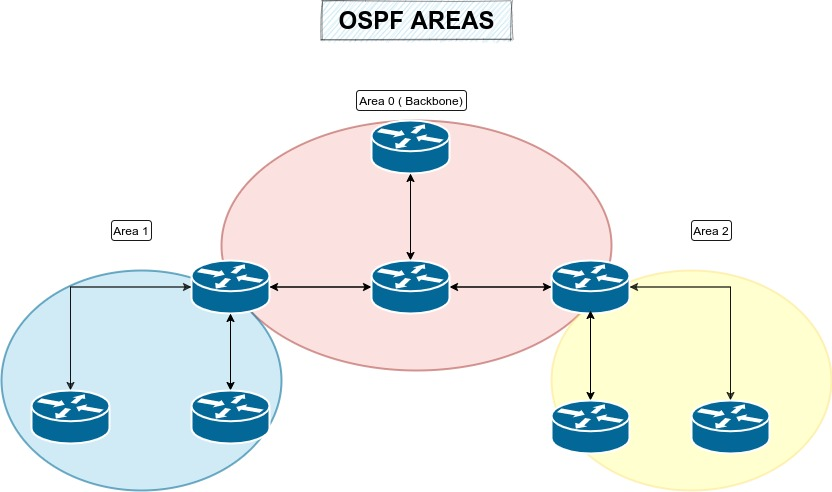
\includegraphics[width=1\linewidth]{fig/OSPFArea.png}
    \caption{OSPF - Áreas}
    \label{fig:OSPFArea}
\end{figure}

Como a figura \ref{fig:OSPFArea} demonstra, uma prática comum, principalmente na área 0, é a ocorrência de roteadores com múltiplas interfaces localizados em diferentes áreas, ou seja, cada interface em uma área diferente. Neste caso, o roteador irá manter uma base de dados da topologia para cada área. Esse é o caso dos roteadores 2, 4 e 7.

O protocolo OSPF funciona utilizando um algoritmo do tipo Link State, o que aumenta a sua complexidade, mas permite uma fácil e eficiente detecção de falhas.

\subsection{VLANS}
Uma VLAN (Virtual Local Area Network ou Rede Local Virtual) é uma tecnologia que permite segmentar uma rede física em várias redes lógicas independentes dentro do mesmo switch. Ela isola o tráfego de dispositivos, aumentando a segurança, o desempenho e facilitando a administração, permitindo agrupar usuários por função, independentemente da localização física.

Cada porta do switch pode ser configurada nas seguintes formas:

\begin{itemize}
    \item Access Port: geralmente são portas conectadas aos dispositivos finais, como PCs, impressoras e servidores.
    \item Trunk Port: normalmente são usadas em uplinks entre switches. Esse tipo de porta transporta frames com a devida identificação de VLAN (tagging), de um switch para outro na rede.
\end{itemize}

A Figura \ref{fig:VLANSMode} representa as seguintes formas de configuração do switch.

\begin{figure}[H]
    \centering
    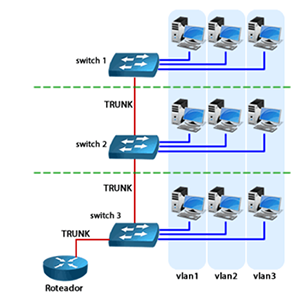
\includegraphics[width=1\linewidth]{fig/VLANSMode.png}
    \caption{Modos de Portas do Switch}
    \label{fig:VLANSMode}
\end{figure}

\subsection{Servidor Web}
O servidor web é um computador que basicamente entrega conteúdo da web para os usuários. Ele faz o armazenamento, processamento e entrega dos arquivos dos sites para os navegadores. Ele também é responsável por processar as requisições de FTP.

\subsection{Network Address Translation}
A Network Address Translation (NAT) \cite{rfc3022} é uma técnica comumente usada por provedores de serviços de internet (ISPs) e organizações para permitir que vários dispositivos compartilhem um único endereço IP público. Ao usar NAT, os dispositivos em uma rede privada podem se comunicar com dispositivos em uma rede pública sem a necessidade de que cada dispositivo tenha seu próprio endereço IP exclusivo.

\subsection{Protocolo Secure Shell - SSH}
O protocolo Secure Shell (SSH) \cite{ssh} é um protocolo para controlar servidores remotamente, gerenciar a infraestrutura e transferir arquivos. Por meio desse protocolo, é possível enviar comandos de forma segura, autenticar e criptografar conexões entre dispositivos.

\subsection{Secure Copy Protocol}
O Secure Copy Protocol (SCP) \cite{scp} é um método baseado no Secure Shell - SSH para transferir arquivos de computador com segurança entre um host local e um host remoto, ou entre dois hosts remotos.

\subsection{Protocolo de transferência de arquivos}

O Protocolo de transferência de arquivos (FTP) é um protocolo de rede padrão usado para a transferência de arquivos de um host para outro em uma rede baseada em TCP, como a Internet \cite{ftp}.

\subsection{Protocolo SNMP}

O \textit{Simple Network Management Protocol} (SNMP) é um protocolo amplamente utilizado para o gerenciamento e monitoramento de dispositivos em redes de computadores. Ele permite que administradores acompanhem o estado e o desempenho de equipamentos como roteadores, switches e servidores de forma centralizada e padronizada \cite{stallings_snmp}.

O funcionamento do SNMP baseia-se em um modelo de comunicação entre um \textit{manager} (gerente) e múltiplos \textit{agents} (agentes). O manager é responsável por solicitar informações ou configurar parâmetros, enquanto os agents são executados nos dispositivos gerenciados e respondem às requisições. As informações são organizadas em uma estrutura hierárquica chamada MIB (\textit{Management Information Base}).

Além das requisições diretas, o SNMP também permite o envio de notificações assíncronas, conhecidas como \textit{traps}, que alertam o manager sobre eventos importantes, como falhas ou mudanças no estado do dispositivo. Isso torna o protocolo essencial para a detecção rápida de problemas e manutenção da qualidade de serviço em redes.

Apesar de sua eficiência e simplicidade, versões mais antigas do SNMP apresentam limitações em relação à segurança. A versão SNMPv3 foi desenvolvida para suprir essas limitações, oferecendo recursos de autenticação e criptografia \cite{rfc3411}.


\subsection{Firewall}

Os firewalls podem ser vistos como barreiras ou gateways que gerenciam o percurso de 
atividades da Web permitidas e proibidas em uma rede privada.  Os firewalls de segurança de 
rede são usados para gerenciamento de tráfego da Web. Normalmente, são destinados a retardar 
a propagação de ameaças da Web.

Para segmentar uma rede são utilizados computadores de gateway especializados chamados de 
roteadores de filtragem. Os firewalls podem ser divididos em:

\begin{itemize}
    \item \textbf{Firewall de rede:} é posicionado na junção entre redes confiáveis e não confiáveis, 
    como sistemas internos e a Internet, Figura \ref{fig:network-firewall}. Sua função principal é monitorar, controlar e decidir sobre a validade do 
    tráfego de entrada e saída com base em um conjunto predefinido de regras. Essas regras foram criadas para 
    impedir o acesso não autorizado e manter a integridade da rede.

    \item \textbf{Firewall baseado em host:} 
    Um firewall de software baseado em host é um software que opera em um único dispositivo dentro de uma rede, 
    Figura \ref{fig:host-based-firewall}.
     Ele é instalado diretamente em computadores ou dispositivos individuais, oferecendo uma camada específica de 
     proteção contra possíveis ameaças. Ao examinar o tráfego de entrada e saída desse dispositivo específico, ele 
     filtra efetivamente o conteúdo nocivo, garantindo que malware, vírus e outras atividades mal-intencionadas não se 
     infiltrem no sistema.
    
\end{itemize}


\begin{figure}[H]
    \centering
    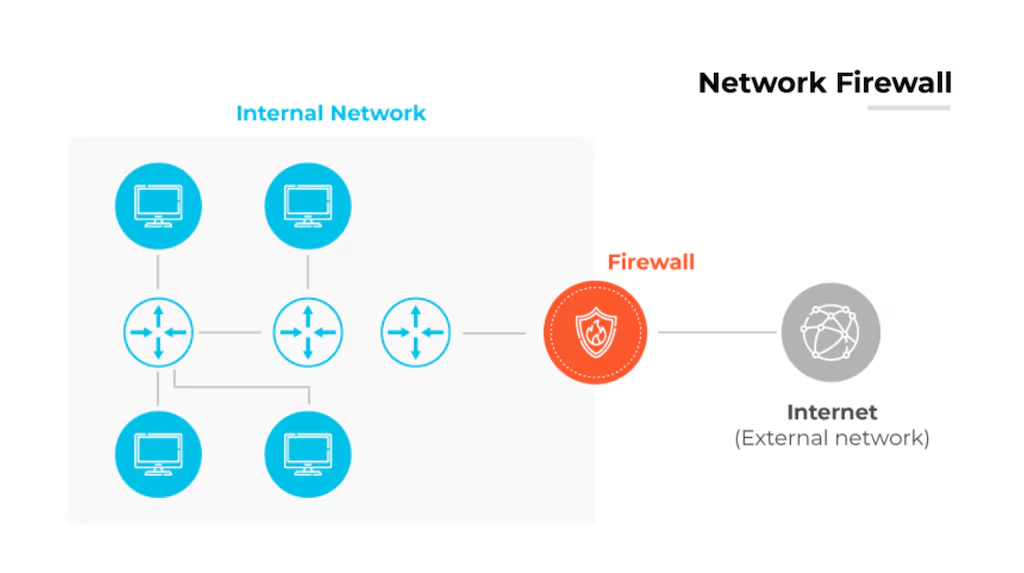
\includegraphics[width=1\linewidth]{fig/network-firewall.png}
    \caption{Firewall de rede}
    \label{fig:network-firewall}
\end{figure}

\begin{figure}[H]
    \centering
    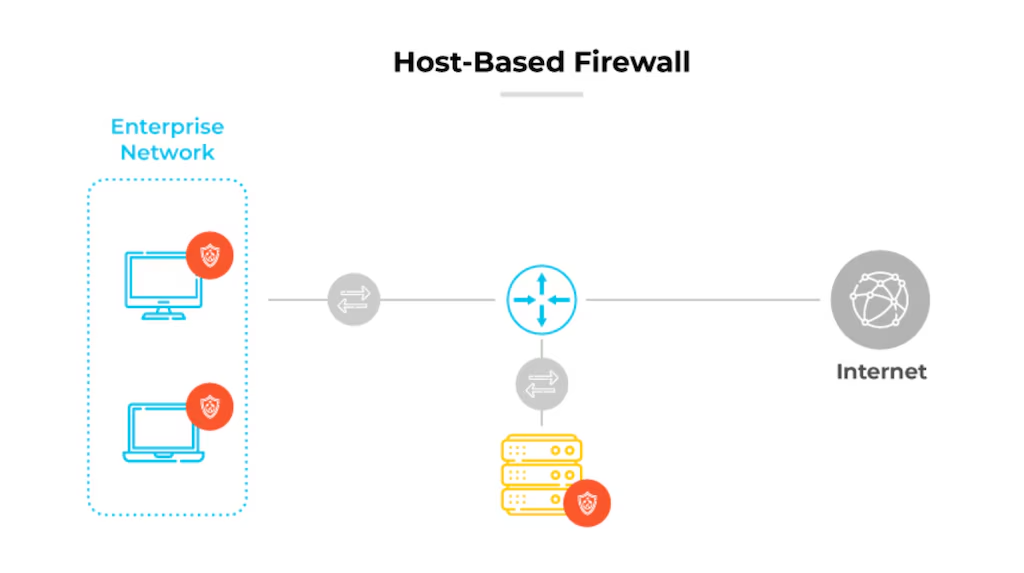
\includegraphics[width=1\linewidth]{fig/host-based-firewall.png}
    \caption{Firewall baseado em host}
    \label{fig:host-based-firewall}
\end{figure}



%------------------------------------------------------------------------
\section{Aplicações Utilizadas}

\subsection{PNETLab}

Para a implementação da rede de infraestrutura, foi utilizado o ambiente virtual PNETLab\cite{pnetlab}. Essa plataforma permite a criação de cenários complexos com roteadores, switches e hosts, possibilitando a simulação de infraestruturas reais de rede.

O PNETLab foi empregado para configurar e interligar os dispositivos da topologia, executar os comandos de configuração e realizar testes de conectividade entre os nós da rede. Dessa forma, foi possível analisar o comportamento do sistema e validar o funcionamento dos protocolos e serviços implementados, como VLANs, OSPF e NAT, sem a necessidade de equipamentos físicos.

\subsubsection{IpTables}

O Iptables é uma ferramenta de firewall utilizada em sistemas Linux para controlar e filtrar o tráfego de rede. Por meio de regras definidas pelo administrador, é possível permitir ou bloquear conexões, aumentando a segurança da rede e do sistema. Seu funcionamento é baseado em tabelas e cadeias (\textit{chains}) responsáveis pelo tratamento dos pacotes. As principais tabelas são: \begin{itemize} \item \textbf{Filter:} utilizada para permitir ou bloquear pacotes de entrada, saída e encaminhamento. \item \textbf{NAT:} responsável pela tradução de endereços IP, sendo utilizada em mascaramento e redirecionamento de portas. \item \textbf{Mangle:} utilizada para modificar informações dos pacotes de rede. \end{itemize}

Em conclusão, o Iptables é uma ferramenta essencial para segurança e gerenciamento de redes em sistemas Linux. 
Sua estrutura baseada em tabelas e cadeias permite controlar o tráfego de forma eficiente, possibilitando a criação 
de regras para filtragem, tradução de endereços e manipulação de pacotes. Dessa forma, o Iptables contribui para 
a proteção, organização e controle das comunicações em ambientes computacionais.


\subsubsection{UFW}

O UFW (\textit{Uncomplicated Firewall}) é uma ferramenta de gerenciamento de firewall desenvolvida para simplificar a configuração de regras de segurança em sistemas Linux. Ele funciona como uma interface mais simples para o Iptables, permitindo que o usuário configure políticas de rede por meio de comandos mais intuitivos e de fácil utilização.

Com o UFW, é possível permitir ou bloquear conexões de entrada e saída, controlar portas específicas e definir regras para diferentes serviços de rede. Sua utilização é bastante comum em servidores Linux devido à facilidade de configuração e ao rápido gerenciamento das regras de firewall.

Além disso, o UFW oferece suporte tanto para protocolos IPv4 quanto IPv6, contribuindo para uma administração mais completa da segurança da rede. Dessa forma, a ferramenta se destaca por proporcionar uma maneira prática e eficiente de implementar políticas de controle de tráfego e proteção em sistemas computacionais.


\subsection{Iperf3}
O iPerf3 é uma ferramenta para medições ativas da largura de banda máxima alcançável
 em redes IP. Ele suporta o ajuste de vários parâmetros relacionados a temporização, buffers e protocolos (TCP, UDP, SCTP com IPv4 e IPv6). Para cada teste, ele reporta a largura de banda, a perda de pacotes e outros parâmetros.

\subsection{NMAP}

O Nmap ("Mapeador de Rede") é um utilitário gratuito e de código aberto para descoberta de redes e auditoria de segurança. Muitos administradores de sistemas e redes também o consideram útil para tarefas como inventário de rede, gerenciamento de cronogramas de atualização de serviços e monitoramento do tempo de atividade de hosts ou serviços. O Nmap utiliza pacotes IP brutos de maneiras inovadoras para determinar quais hosts estão disponíveis na rede, quais serviços (nome e versão do aplicativo) esses hosts oferecem, quais sistemas operacionais (e versões do SO) estão em execução, que tipo de filtros de pacotes/firewalls estão em uso e dezenas de outras características. Ele foi projetado para escanear rapidamente grandes redes, mas funciona bem com hosts individuais. 

\subsection{SNORT}

O Snort é o principal Sistema de Prevenção de Intrusões (IPS) de código aberto do mundo. O Snort IPS utiliza uma série de regras que ajudam a definir atividades maliciosas na rede e usa essas regras para encontrar pacotes que correspondam a elas, gerando alertas para os usuários.

O Snort também pode ser implementado em linha para bloquear esses pacotes. O Snort tem três usos principais: como um analisador de pacotes, semelhante ao tcpdump; como um registrador de pacotes — útil para depuração de tráfego de rede; ou como um sistema completo de prevenção de intrusões em redes. 
%-------------------------------------------------------------------------
\section{Topologia}

Para este laboratório, teremos os seguintes dispositivos: 4 roteadores (VYOS), 3 switches (EXOS), 2 Ubuntu, 1 servidor Zabbix, 1 PC Windows e 2 VPCs, como mostrado na Figura \ref{fig:topologia}.

\begin{figure*}[t]
    \centering
    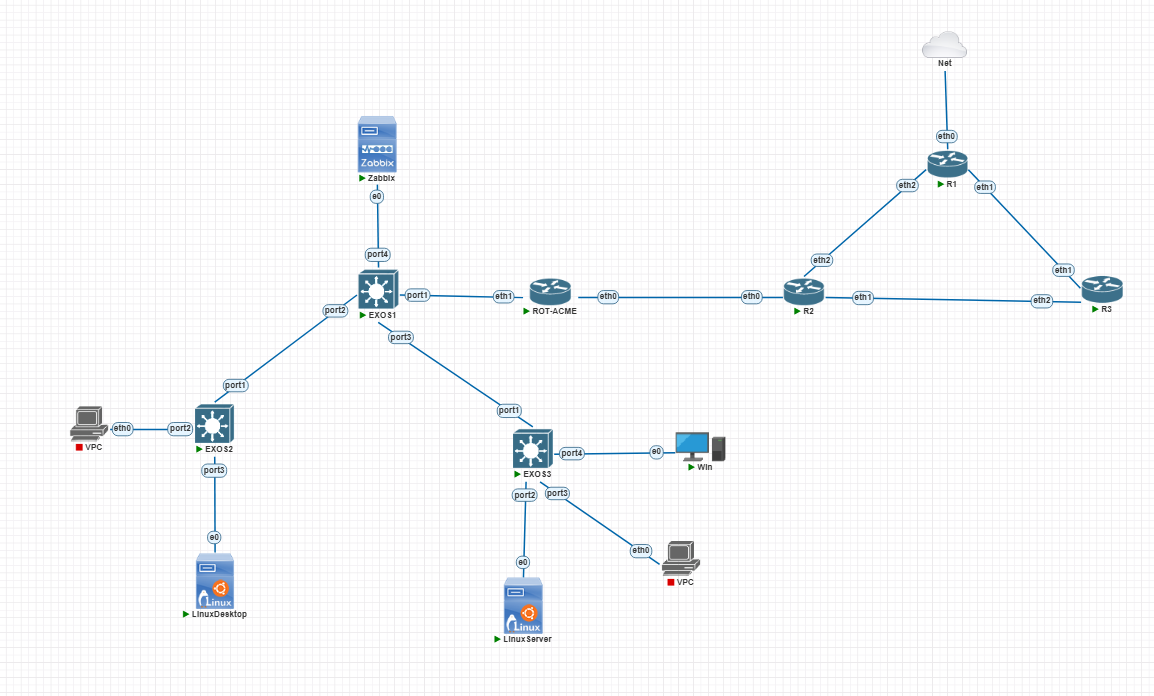
\includegraphics[width=\textwidth]{fig/topologia.png}
    \caption{Topologia}
    \label{fig:topologia}
\end{figure*}

Na Figura \ref{fig:roteadorP1}, temos os roteadores R1, R2 e R3, com a topologia em anel.

\begin{figure}[H]
    \centering
    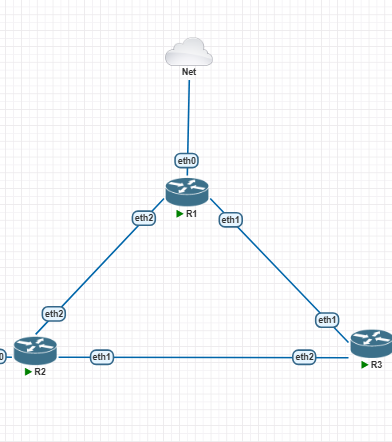
\includegraphics[width=1\linewidth]{fig/roteadorP1.png}
    \caption{Roteadores R1, R2 e R3}
    \label{fig:roteadorP1}
\end{figure}

\subsection{Roteador R1}

Para o roteador R1, temos a seguinte tabela de roteamento \ref{tab:routingR1}.

\begin{table}[h]
    \centering
    \begin{tabular}{c|c|c|c}
        Interface & Destino & Máscara \\
        \hline
        eth0 & Via DHCP & Via DHCP \\
        eth1 & 192.168.15.1 & 255.255.255.240 \\
        eth2 & 192.168.15.17 & 255.255.255.240 \\
    \end{tabular}
    \caption{Tabela de roteamento R1}
    \label{tab:routingR1}
\end{table}

\subsection{Roteador R2}

Para o roteador R2, temos a seguinte tabela de roteamento \ref{tab:routingR2}.

\begin{table}[h]
    \centering
    \begin{tabular}{c|c|c|c}
        Interface & Destino & Máscara \\
        \hline
        eth0 & 192.168.15.30 & 255.255.255.240 \\
        eth1 & 192.168.15.33 & 255.255.255.240 \\
    \end{tabular}
    \caption{Tabela de roteamento R2}
    \label{tab:routingR2}
\end{table}

\subsection{Roteador R3}

Para o roteador R3, temos a seguinte tabela de roteamento \ref{tab:routingR3}.

\begin{table}[h]
    \centering
    \begin{tabular}{c|c|c|c}
        Interface & Destino & Máscara \\
        \hline
        eth1 & 192.168.15.46 & 255.255.255.240 \\
        eth2 & 192.168.15.50 & 255.255.255.240 \\
    \end{tabular}
    \caption{Tabela de roteamento R3}
    \label{tab:routingR3}
\end{table}

\subsection{Roteador ROT-ACME}
O roteador ROT-ACME, mostrado na Figura \ref{fig:roteadorROT}, interliga a rede local com os roteadores da topologia em anel.

\begin{figure}[H]
    \centering
    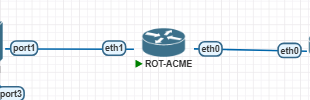
\includegraphics[width=1\linewidth]{fig/roteadorROT.png}
    \caption{Roteador ROT-ACME}
    \label{fig:roteadorROT}
\end{figure}

A Tabela \ref{tab:routingROTACME} representa a tabela de roteamento do ROT-ACME.

\begin{table}[h]
    \centering
    \begin{tabular}{c|c|c|c}
        Interface & Destino & Máscara \\
        \hline
        eth0 & 192.168.15.14 & 255.255.255.240 \\
        eth1 & 172.24.1.254 & 255.255.255.0 \\
    \end{tabular}
    \caption{Tabela de roteamento ROT-ACME}
    \label{tab:routingROTACME}
\end{table}


%-------------------------------------------------------------------------
\section{Configuração}

Para a realização deste laboratório, foram configurados os dispositivos de rede com o objetivo de permitir a comunicação entre diferentes sub-redes, o gerenciamento pelo SNMP e o acesso à rede externa.

\subsection{Roteadores}
\subsubsection{Roteador ROT-ACME}

No roteador ROT-ACME, utilizando o sistema operacional VyOS, foram configuradas as interfaces de rede física e virtual (VLANs), atribuindo endereços IP para cada segmento da rede. Além disso, foi definida uma rota padrão para encaminhamento de tráfego externo, implementado o SNMP e o NAT, permitindo o gerenciamento de redes e que as redes internas acessem outras redes por meio da interface de saída. As configurações realizadas podem ser observadas no Código~\ref{lst:rotacme}.

\subsubsection{Roteador R1}

No roteador R1, foram configuradas as interfaces de rede com endereçamento dinâmico na interface de acesso externo e endereçamento estático nas interfaces internas. Além disso, foi implementado o protocolo de roteamento dinâmico OSPF, permitindo a troca de rotas entre os roteadores do backbone. Também foi configurado o NAT para possibilitar o acesso à rede externa, bem como a redistribuição de rotas conectadas. Além disso, foi configurado o protocolo SNMP para permitir o gerenciamento do dispositivo. As configurações realizadas podem ser observadas no Código~\ref{lst:rotR1}.

\subsubsection{Roteador R2}
O roteador R2 foi configurado com endereçamento IP em suas interfaces de rede, interligando diferentes sub-redes do backbone. Assim como no R1, foi utilizado o protocolo OSPF para permitir o roteamento dinâmico entre os dispositivos da rede. Foi configurada uma interface de loopback para identificação do roteador no processo de roteamento, além da redistribuição de rotas conectadas. Também foi configurado o protocolo SNMP para permitir o gerenciamento do dispositivo. As configurações realizadas podem ser observadas no Código~\ref{lst:rotR2}.

\subsubsection{Roteador R3}
No roteador R3, foram configuradas as interfaces de rede responsáveis pela interconexão com outras sub-redes do backbone. O protocolo OSPF foi implementado para permitir a comunicação e troca de informações de roteamento com os demais roteadores. Além disso, foi definida uma identificação única por meio de uma interface de loopback, garantindo a correta operação do protocolo. Também foi configurado o protocolo SNMP para permitir o gerenciamento do dispositivo. As configurações realizadas podem ser observadas no Código~\ref{lst:rotR3}.

\subsection{Switches}

\subsubsection{Switch EXOS1}

No switch EXOS1, foram criadas e configuradas as VLANs correspondentes à rede, incluindo a VLAN de gerenciamento. As portas foram configuradas como trunk para permitir a passagem de múltiplas VLANs entre dispositivos e como acesso para conexão de hosts finais. Também foi atribuído um endereço IP para gerenciamento do equipamento, definida uma rota padrão para comunicação externa e a configuração do SNMP. As configurações realizadas podem ser observadas no Código~\ref{lst:exos1}.

\subsubsection{Switch EXOS2}
O switch EXOS2 foi configurado com VLANs associadas aos diferentes setores da rede, com portas configuradas em modo trunk e acesso conforme a necessidade da topologia. As configurações garantem a comunicação adequada entre os dispositivos conectados e a segmentação lógica da rede. Também foi atribuído um endereço IP para gerenciamento do equipamento, definida uma rota padrão para comunicação externa e a configuração do SNMP. As configurações realizadas podem ser observadas no Código~\ref{lst:exos2}.

\subsubsection{Switch EXOS3}
No switch EXOS3, foram realizadas configurações semelhantes às dos demais switches, com a criação de VLANs e associação de portas em modo trunk e acesso. Essa configuração permite a integração do switch à topologia da rede, garantindo a comunicação entre os diferentes segmentos configurados. Por fim, foi atribuído um endereço IP para gerenciamento do equipamento, definida uma rota padrão para comunicação externa e a configuração do SNMP. As configurações realizadas podem ser observadas no Código~\ref{lst:exos3}.

\subsection{Servidor Zabbix}

A configuração do servidor Zabbix foi realizada com base na documentação oficial do Zabbix\cite{zabbix_install}. Inicialmente, foi realizada a configuração do endereço IP estático do servidor por meio do arquivo \texttt{/etc/netplan/01-network-manager-all.yaml}, conforme apresentado no Código \ref{lst:ZabbixServerIp}.

\begin{listing}[H]
\centering
\begin{minted}[
    bgcolor=bgcolor,
    frame=lines,
    breaklines=true,
    breakanywhere=true,
    fontsize=\footnotesize,
]{yaml}

network:
  version: 2
  renderer: networkd

  ethernets:
    ens3:
      dhcp4: no
      addresses:
        - 172.24.30.4/24
      routes:
        - to: default
          via: 172.24.30.254
      nameservers:
        addresses:
          - 8.8.8.8

\end{minted}
\caption{Configuração do IP - Servidor Zabbix}
\label{lst:ZabbixServerIp}
\end{listing}

Após a configuração do endereço IP, foi realizada a instalação do servidor Zabbix seguindo os procedimentos descritos na documentação oficial. Durante a configuração, foram realizadas alterações no arquivo \texttt{/etc/zabbix/zabbix\_server.conf}, conforme apresentado no Código \ref{lst:ZabbixServerConf}.

\begin{listing}[H]
\centering
\begin{minted}[
    bgcolor=bgcolor,
    frame=lines,
    breaklines=true,
    breakanywhere=true,
    fontsize=\footnotesize,
]{yaml}

DBName=zabbix
DBUser=zabbix
DBPassword=zabbix

\end{minted}
\caption{Configuração do arquivo zabbix\_server.conf}
\label{lst:ZabbixServerConf}
\end{listing}

Por fim, os serviços do servidor Zabbix, Nginx e banco de dados foram reiniciados para aplicação das configurações realizadas, conforme mostrado no Código \ref{lst:ZabbixRestart}.

\begin{listing}[H]
\centering
\begin{minted}[
    bgcolor=bgcolor,
    frame=lines,
    breaklines=true,
    breakanywhere=true,
    fontsize=\footnotesize,
]{bash}

sudo systemctl restart zabbix-server
sudo systemctl restart nginx
sudo systemctl restart mysql

\end{minted}
\caption{Reinicialização dos serviços do servidor Zabbix}
\label{lst:ZabbixRestart}
\end{listing}

\subsection{Linux}

\subsubsection{Linux Server}
Para esse dispositivo, foi feita a configuração dos IPs e do DNS por meio do arquivo \textit{/etc/netplan/01-network-manager-all.yaml}. Nesse arquivo, foram adicionadas as configurações mostradas no Código \ref{lst:LinuxServerIp}.

\begin{listing}[H]
\centering
\begin{minted}[
    bgcolor=bgcolor,
    frame=lines,
    breaklines=true,
    breakanywhere=true,
    fontsize=\footnotesize,
]{yaml}

network:
  version: 2
  renderer: networkd

  ethernets:
    ens3:
      dhcp4: no
      addresses:
        - 172.24.10.2/24
      routes:
        - to: default
          via: 172.24.10.254
      nameservers:
        addresses:
          - 172.16.4.2

\end{minted}
\caption{Configuração do IP - Linux Server}
\label{lst:LinuxServerIp}
\end{listing}

Além da configuração do IP, foi feita a instalação do servidor web - Nginx, como mostrado no Código \ref{lst:LinuxServerWeb}.

\begin{listing}[H]
\centering
\begin{minted}[
    bgcolor=bgcolor,
    frame=lines,
    breaklines=true,
    breakanywhere=true,
    fontsize=\footnotesize,
]{bash}

sudo apt install nginx -y

\end{minted}
\caption{Instalação do servidor web - Linux Server}
\label{lst:LinuxServerWeb}
\end{listing}

Por fim, foi instalado o Zabbix Agent, utilizado para monitoramento do dispositivo pelo servidor Zabbix. Após a instalação, foi realizada a configuração do endereço do servidor responsável pela coleta das métricas e a definição do hostname do equipamento.

A configuração foi realizada no arquivo \texttt{/etc/zabbix/zabbix\_agentd.conf}, conforme apresentado no Código \ref{lst:LinuxServerZabbixAgent}.

\begin{listing}[H]
\centering
\begin{minted}[
    bgcolor=bgcolor,
    frame=lines,
    breaklines=true,
    breakanywhere=true,
    fontsize=\footnotesize,
]{yaml}

Server=172.24.30.4
ServerActive=172.24.30.4
Hostname=LinuxServer

\end{minted}
\caption{Configuração do Zabbix Agent - Linux Server}
\label{lst:LinuxServerZabbixAgent}
\end{listing}

Após a configuração, o serviço do agente foi reiniciado para aplicação das alterações realizadas.

\begin{listing}[H]
\centering
\begin{minted}[
    bgcolor=bgcolor,
    frame=lines,
    breaklines=true,
    breakanywhere=true,
    fontsize=\footnotesize,
]{bash}

sudo systemctl restart zabbix-agent
sudo systemctl enable zabbix-agent

\end{minted}
\caption{Inicialização do serviço Zabbix Agent}
\label{lst:LinuxServerZabbixRestart}
\end{listing}

\subsubsection{Linux Desktop}
Para esse dispositivo, foi feita a configuração dos IPs e do DNS por meio do arquivo \textit{/etc/netplan/01-network-manager-all.yaml}. Nesse arquivo, foram adicionadas as configurações mostradas no Código \ref{lst:LinuxDesktopIp}.

\begin{listing}[H]
\centering
\begin{minted}[
    bgcolor=bgcolor,
    frame=lines,
    breaklines=true,
    breakanywhere=true,
    fontsize=\footnotesize,
]{yaml}

network:
  version: 2
  renderer: networkd

  ethernets:
    ens3:
      dhcp4: no
      addresses:
        - 172.24.10.3/24
      routes:
        - to: default
          via: 172.24.10.254
      nameservers:
        addresses:
          - 172.16.4.2

\end{minted}
\caption{Configuração do IP - Linux Desktop}
\label{lst:LinuxDesktopIp}
\end{listing}

Por fim, foi instalado o Zabbix Agent, utilizado para monitoramento do dispositivo pelo servidor Zabbix. Após a instalação, foi realizada a configuração do endereço do servidor responsável pela coleta das métricas e a definição do hostname do equipamento.

A configuração foi realizada no arquivo \texttt{/etc/zabbix/zabbix\_agentd.conf}, conforme apresentado no Código \ref{lst:LinuxDesktopZabbixAgent}.

\begin{listing}[H]
\centering
\begin{minted}[
    bgcolor=bgcolor,
    frame=lines,
    breaklines=true,
    breakanywhere=true,
    fontsize=\footnotesize,
]{yaml}

Server=172.24.30.4
ServerActive=172.24.30.4
Hostname=LinuxDesktop

\end{minted}
\caption{Configuração do Zabbix Agent - Linux Desktop}
\label{lst:LinuxDesktopZabbixAgent}
\end{listing}

Após a configuração, o serviço do agente foi reiniciado para aplicação das alterações realizadas.

\begin{listing}[H]
\centering
\begin{minted}[
    bgcolor=bgcolor,
    frame=lines,
    breaklines=true,
    breakanywhere=true,
    fontsize=\footnotesize,
]{bash}

sudo systemctl restart zabbix-agent
sudo systemctl enable zabbix-agent

\end{minted}
\caption{Inicialização do serviço Zabbix Agent}
\label{lst:LinuxDesktopZabbixRestart}
\end{listing}

\subsection{PC Windows}

Para a configuração do DNS e do IP do PC Windows, foi utilizada a interface do Painel de Controle, como mostrado na Figura \ref{fig:PCWindowsIP}.

\begin{figure}[H]
    \centering
    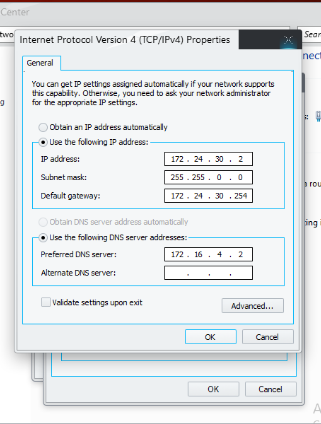
\includegraphics[width=1\linewidth]{fig/PCWindowsIP.png}
    \caption{Configuração IP - PC Windows}
    \label{fig:PCWindowsIP}
\end{figure}

\subsection{VPCs}
Para esse dispositivo, foi feita a configuração dos IPs e do DNS, como mostrado no Código \ref{lst:VPCsIp}.

\begin{listing}[H]
\centering
\begin{minted}[
    bgcolor=bgcolor,
    frame=lines,
    breaklines=true,
    breakanywhere=true,
    fontsize=\footnotesize,
]{bash}

ip 172.24.10.1/24 172.24.10.254
ip dns 172.16.4.2

\end{minted}
\caption{Configuração do IP - VPCs}
\label{lst:VPCsIp}
\end{listing}


%-------------------------------------------------------------------------
\section{Resultados}

\subsection{Envio e Recebimento de dados via Iperf3}

Para esta simulação, foi realizada a transmissão de um arquivo FTP e de um arquivo de voz. Para 
isso foi utilizada a ferramenta Iperf3, com o Host Zabbix atuando como servidor e o Host Linux como cliente. 
O teste de largura de banda entre os hosts foi realizado utilizando o protocolo TCP.

Na primeira simulação, foi realizada a transmissão de um arquivo FTP do Host Linux para o Host Zabbix. Na Figura \ref{fig:iperf2},
 é possível observar o comando utilizado para iniciar o servidor Iperf3 no Host Zabbix, 
 bem como o resultado do teste de largura de banda entre os dois hosts. 
 O teste indicou uma largura de banda de 1 Gbps,
  demonstrando a capacidade da rede para suportar a transferência de arquivos FTP de forma eficiente.


\begin{figure}[H]
    \centering
    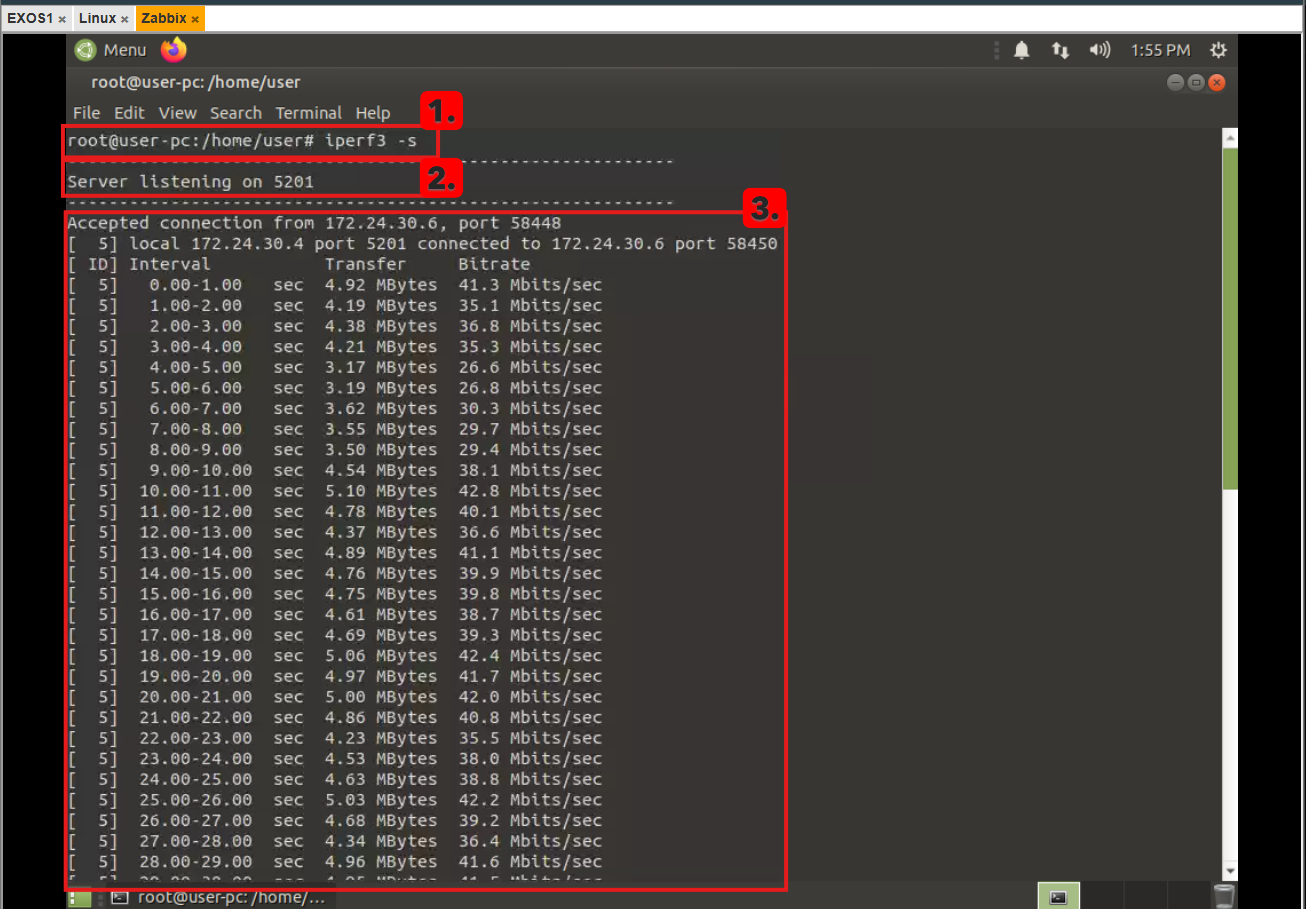
\includegraphics[width=1\linewidth]{fig/iperf2.png}
    \caption{Host Zabbix como servidor Iperf3 - transmissão arquivo FTP; 1. Comando para iniciar o servidor Iperf3; 
    2. Resultado do teste de largura de banda entre o Host Zabbix e o Host Cliente}
    \label{fig:iperf2}
\end{figure}

Na Figura \ref{fig:iperf1}, é possível observar o comando, \textit{iperf3 -c 172.24.30.4 -i 10 -p 5201 -w 8.0K -t 60},
utilizado para iniciar o cliente Iperf3 no Host Linux. O \textit{-c} especifica o endereço IP do servidor, 
\textit{-i} define o intervalo de tempo para exibir os resultados, 
\textit{-p} indica a porta utilizada para a comunicação, 
\textit{-w} define o tamanho da janela TCP e 
\textit{-t} especifica a duração do teste em segundos.

  
Ainda na Figura \ref{fig:iperf1}, é possível ver o resultado do teste de largura de banda entre o Host Linux e o Host Zabbix. 
O teste indicou uma largura de banda de 1 Gbps, confirmando a capacidade da rede para suportar a
transferência de arquivos FTP de forma eficiente.

\begin{figure}[H]
    \centering
    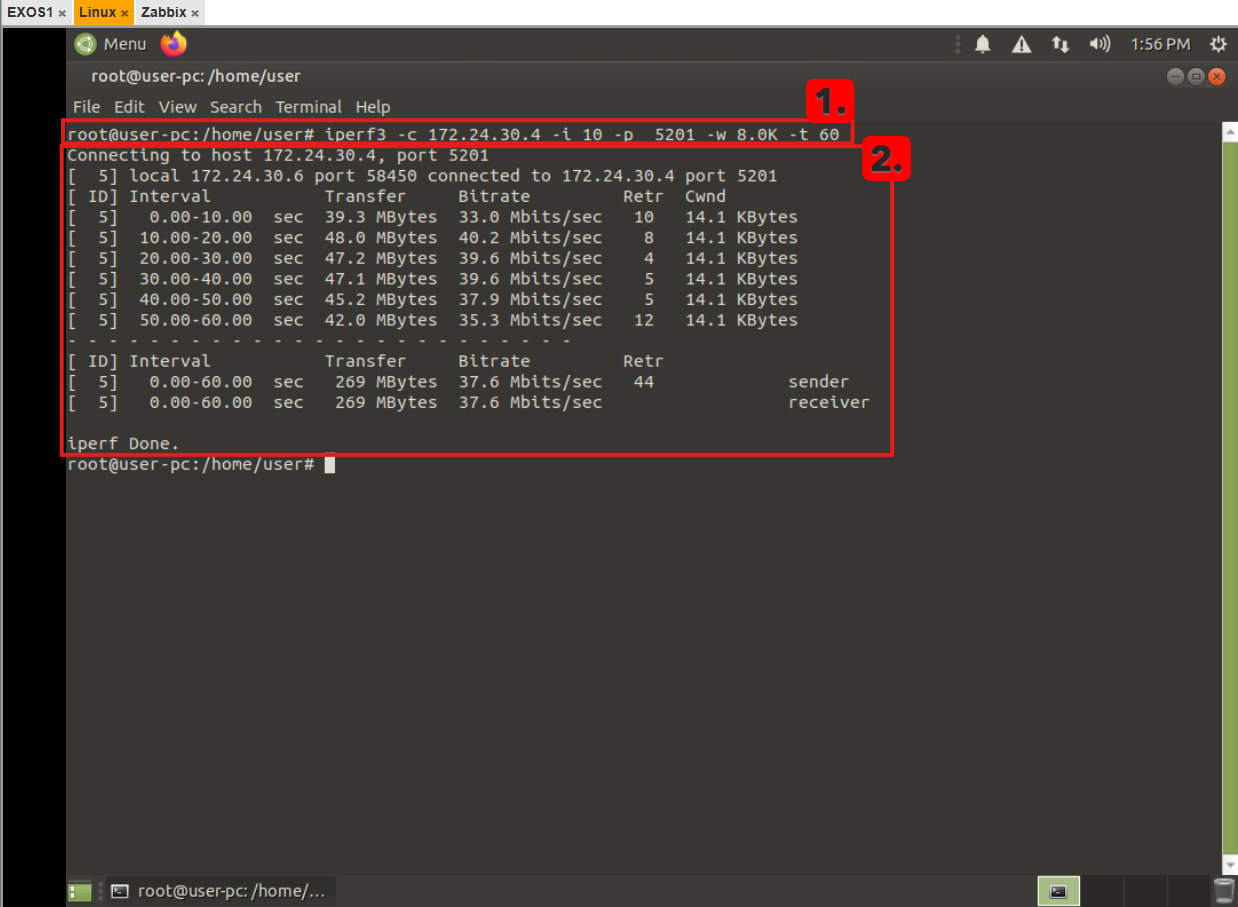
\includegraphics[width=1\linewidth]{fig/iperf1.png}
    \caption{Host Linux como cliente Iperf3 - transmissão arquivo FTP; 1. Comando para iniciar o cliente Iperf3; 
    2. Resultado do teste de largura de banda entre o Host Linux e o Host Zabbix}
    \label{fig:iperf1}
\end{figure}

Já na segunda simulação, foi realizada a transmissão de um arquivo de voz do Host Linux para o Host Zabbix.
Na Figura \ref{fig:iperf3}, é possível observar o comando utilizado para iniciar o servidor Iperf3 no Host Zabbix,
bem como o resultado do teste de largura de banda entre os dois hosts.

\begin{figure}[H]
    \centering
    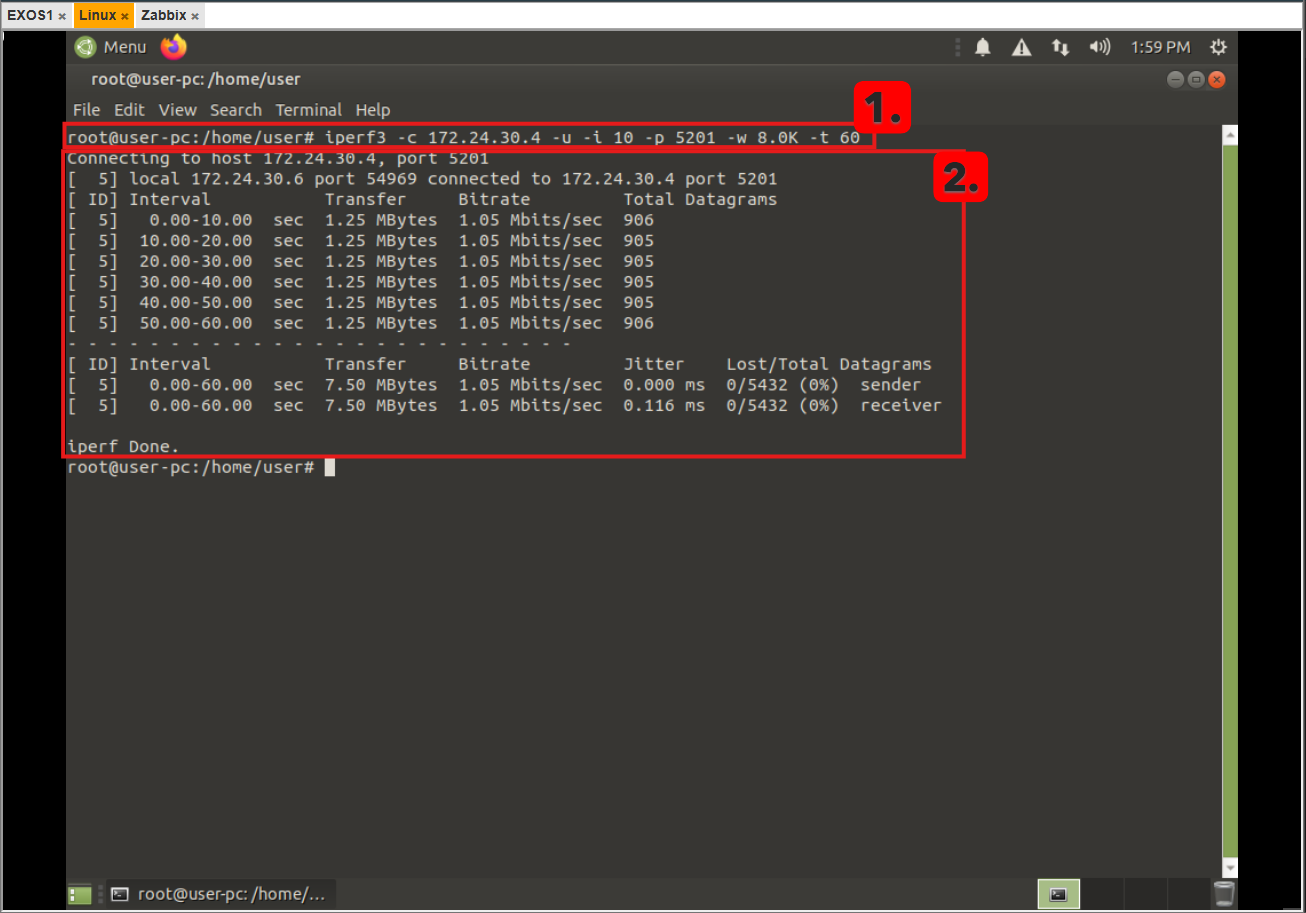
\includegraphics[width=1\linewidth]{fig/iperf3.png}
    \caption{Host Zabbix como servidor Iperf3 - transmissão arquivo de Voz; 1. Comando para iniciar o servidor Iperf3; 
    2. Resultado do teste de largura de banda entre o Host Zabbix e o Host Cliente}
    \label{fig:iperf3}
\end{figure}

Na Figura \ref{fig:iperf4}, é possível observar o comando,\textit{iperf3 -c 172.24.30.4 -u -i 10 -p 5201 -w 8.0K -t 60},
utilizado para iniciar o cliente Iperf3 no Host Linux. No comando, o \textit{-c} especifica o endereço IP do servidor,
O \textit{-u} especifica que o teste deve ser realizado utilizando o protocolo UDP, 
\textit{-i} define o intervalo de tempo para exibir os resultados,
\textit{-p} indica a porta utilizada para a comunicação, 
\textit{-w} define o tamanho da janela TCP e \textit{-t} especifica a duração do teste em segundos.    

Ainda na Figura \ref{fig:iperf4}, é possível ver o resultado do teste de largura de banda entre os dois hosts. O teste indicou uma largura de banda de 1 Gbps,
 demonstrando a capacidade da rede para suportar a transferência de arquivos de voz de forma eficiente.

\begin{figure}[H]
    \centering
    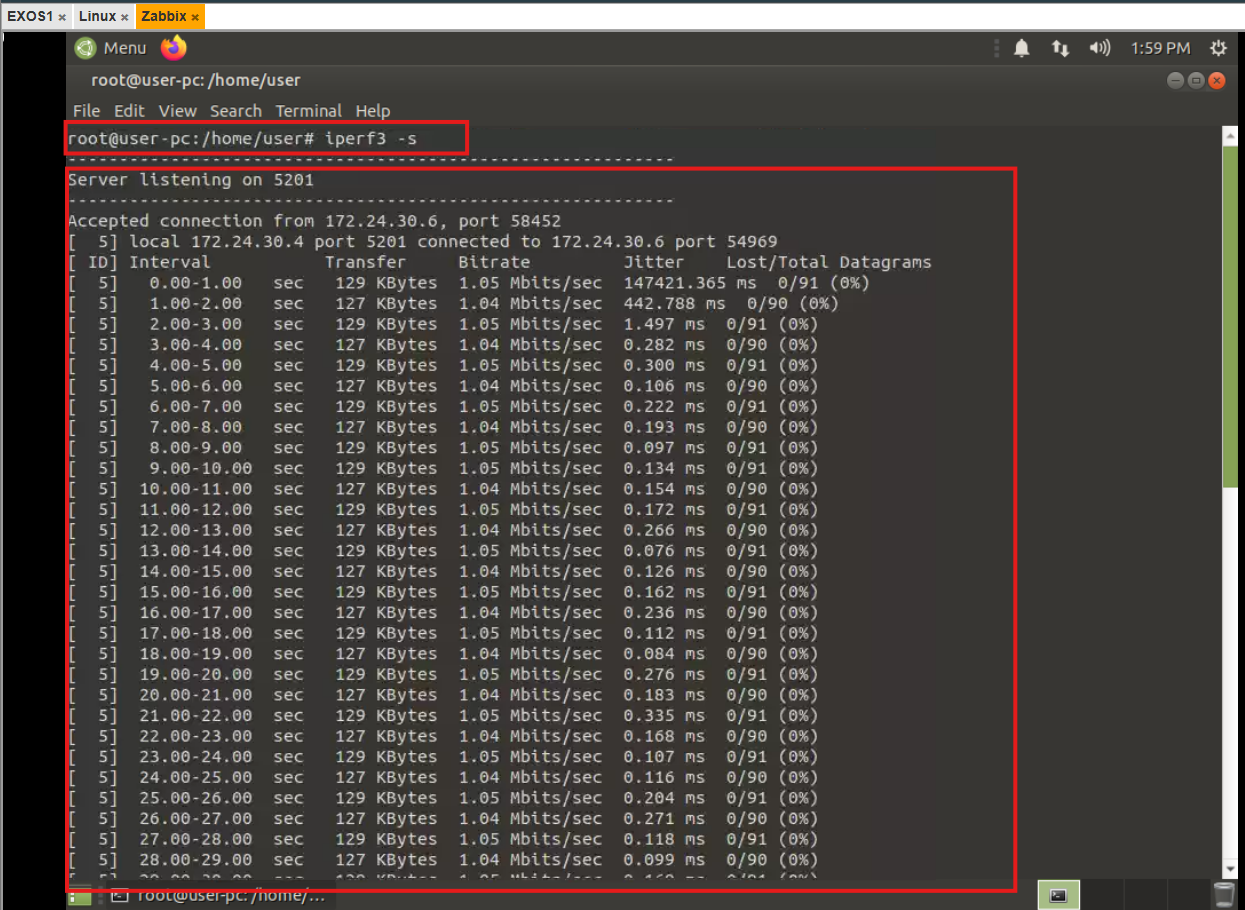
\includegraphics[width=1\linewidth]{fig/iperf4.png}
    \caption{Host Linux como cliente Iperf3 - transmissão arquivo de Voz; 1. Comando para iniciar o cliente Iperf3; 
    2. Resultado do teste de largura de banda entre o Host Linux e o Host Zabbix}
    \label{fig:iperf4}
\end{figure}

\subsection{NMAP}
Para a realização de testes de varredura de portas e identificação de serviços, 
foi utilizada a ferramenta Nmap, como mostrado na Figura \ref{fig:nmap1}. Foi utilizado 
o comando \textit{nmap 172.24.30.4}, que realiza uma varredura de portas 
no endereço IP do Host Zabbix. O resultado da varredura indicou 
que as portas 22 (SSH), 80 (HTTP) e 3306 (MySQL) estavam abertas, indicando a presença desses serviços no Host Zabbix.

\begin{figure}[H]
    \centering
    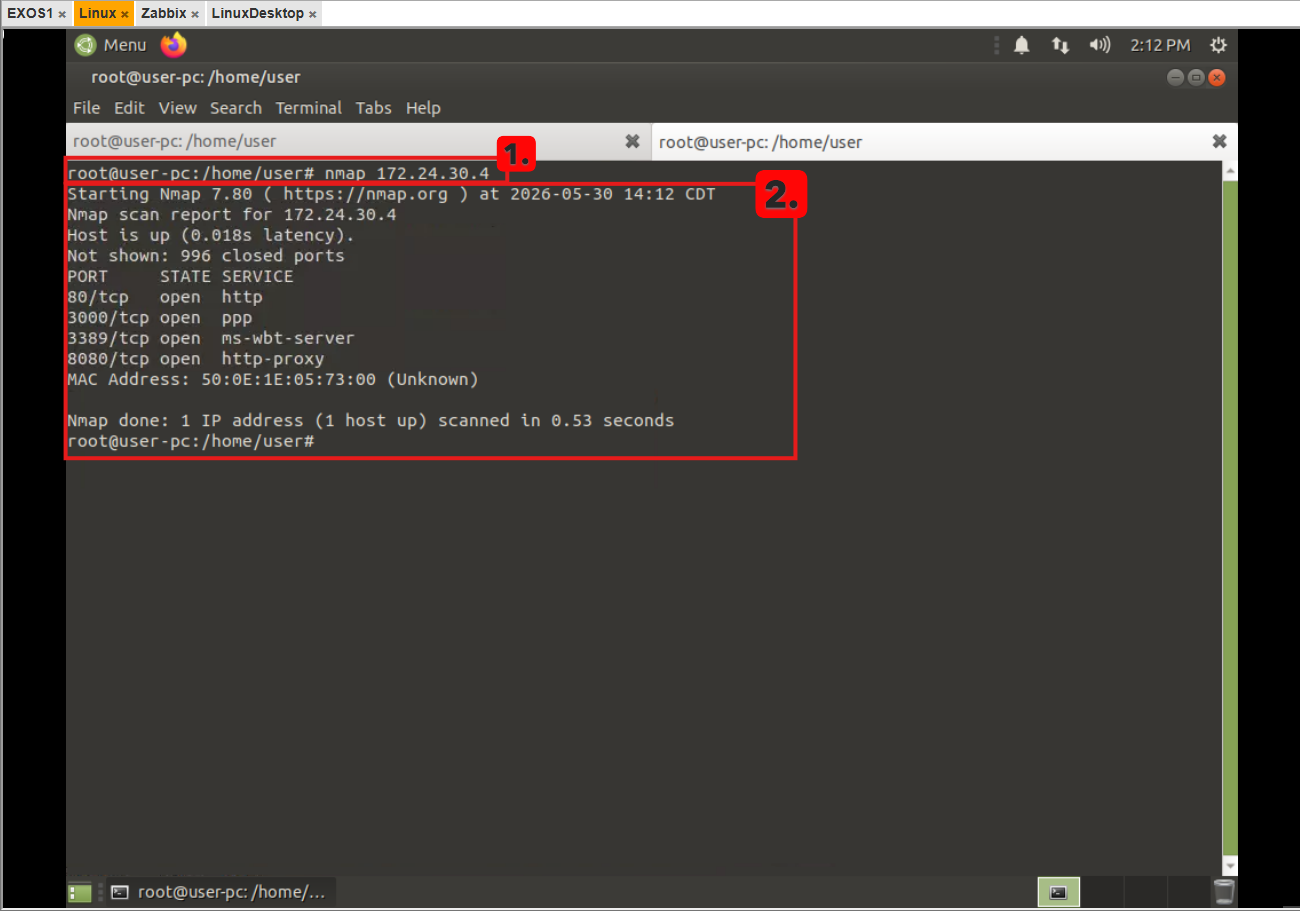
\includegraphics[width=1\linewidth]{fig/nmap1.png}
    \caption{Varredura de portas utilizando o Nmap; 1. Comando para realizar a varredura de portas no Host Zabbix; 
    2. Resultado da varredura indicando as portas abertas e os serviços correspondentes}
    \label{fig:nmap1}
\end{figure}


Já na Figura \ref{fig:nmap2}, foi utilizado o comando, 
\textit{nmap 172.24.30.4 172.24.30.254}, que realiza uma varredura de portas 
nos endereços IPs 172.24.30.4 e 172.24.30.254, 
o resultado da varredura indicou que as portas
22 (SSH), 80 (HTTP) e 3306 (MySQL) estavam abertas no Host Zabbix, 
enquanto as portas dos outros hosts estavam fechadas, indicando a 
ausência desses serviços nos demais hosts da rede.

\begin{figure}[H]
    \centering
    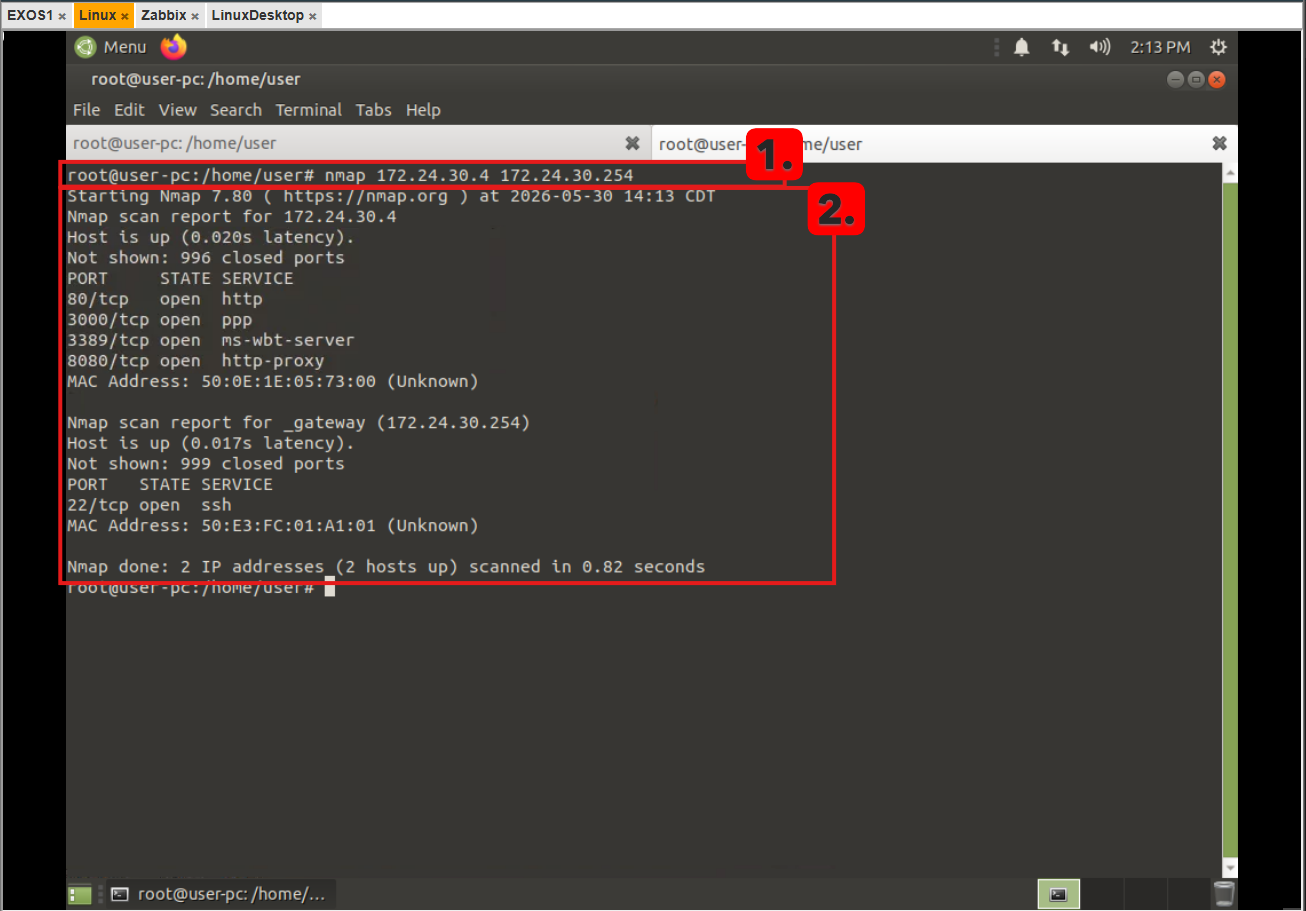
\includegraphics[width=1\linewidth]{fig/nmap2.png}
    \caption{Varredura de portas utilizando o Nmap; 
    1. Comando para realizar a varredura de portas nos endereços IPs 172.24.30.4 e 172.24.30.254; 
    2. Resultado da varredura indicando as portas abertas e os serviços correspondentes}
    \label{fig:nmap2}
\end{figure}

Em seguida, por meio do comando \textit{nmap 172.24.30.1-254}, 
mostrado na Figura \ref{fig:nmap3}, foi realizada 
uma varredura de portas e identificação de serviços em um intervalo de 
endereços IP, o resultado da varredura indicou três endereços IP disponíveis na rede, 
sendo eles 172.30.24.4, 172.30.24.254 e 172.30.24.6. Além disso, a varredura indicou
 quais portas estavam abertas em cada um dos hosts, 
 bem como os serviços correspondentes a essas portas.

\begin{figure}[H]
    \centering
    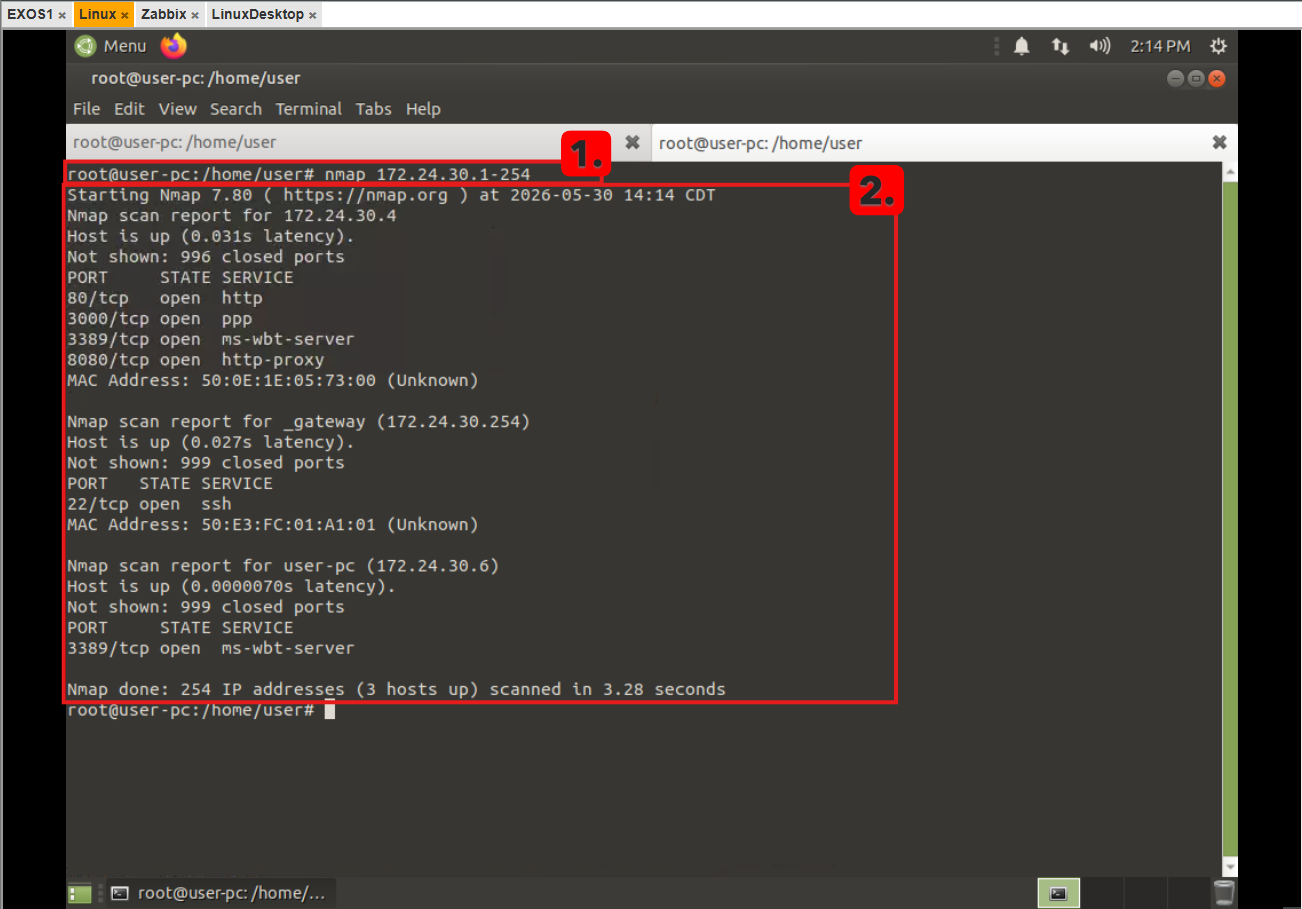
\includegraphics[width=1\linewidth]{fig/nmap3.png}
    \caption{Varredura de portas utilizando o Nmap; 1. Comando para realizar a varredura de portas em um intervalo de endereços IP; 
    2. Resultado da varredura indicando os endereços IP disponíveis na rede, as portas abertas e os serviços correspondentes}
    \label{fig:nmap3}
\end{figure}


Já na Figura \ref{fig:nmap4}, foi utilizado o comando \textit{nmap 172.24.30.254 -sS}, 
que realiza uma varredura de portas utilizando o método de varredura TCP SYN,
 o resultado da varredura indicou que a porta 22 (SSH) estava aberta no gateway e mostrou o MAC Address.

\begin{figure}[H]
    \centering
    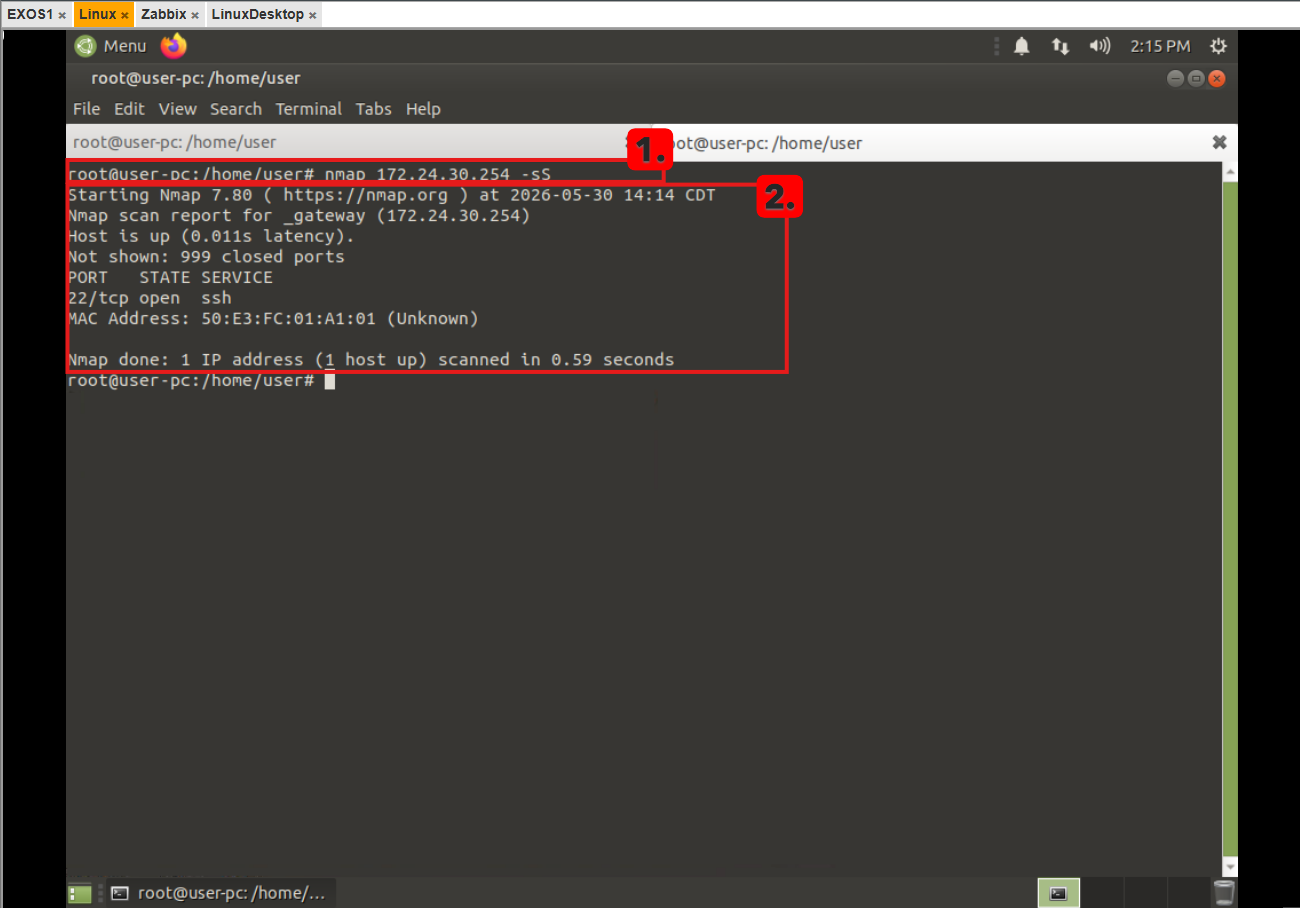
\includegraphics[width=1\linewidth]{fig/nmap4.png}
    \caption{Varredura de portas utilizando o Nmap; 
    1. Comando para realizar a varredura de portas utilizando o método de varredura TCP SYN; 
    2. Resultado da varredura indicando as portas abertas e os serviços correspondentes}
    \label{fig:nmap4}
\end{figure}

Em seguida, por meio do comando \textit{nmap 172.24.30.1-254 -sV}, mostrado na Figura \ref{fig:nmap5},\ref{fig:nmap6} e \ref{fig:nmap7}, 
foi realizada uma varredura de portas e identificação do tipo de serviços utilizando o método de varredura 
TCP SYN em um intervalo de endereços IP, o resultado da varredura indicou quais IPs estavam disponíveis 
na rede, quais portas estavam abertas em cada um dos hosts, 
bem como os serviços e a versão dos serviços correspondentes a essas portas.


\begin{figure}[H]
    \centering
    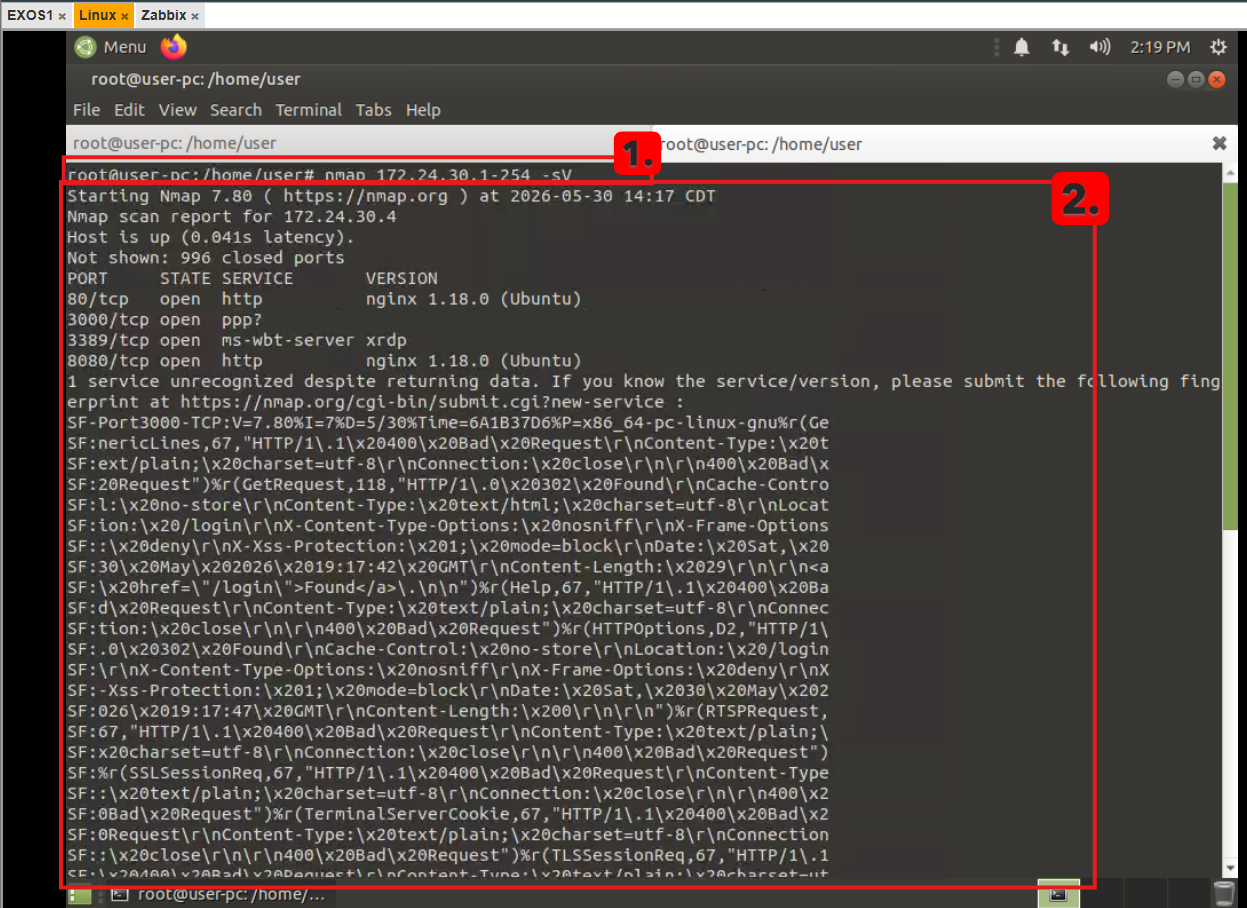
\includegraphics[width=1\linewidth]{fig/nmap5.png}
    \caption{Varredura de portas utilizando o Nmap 1; 
     1. Comando para realizar a varredura de portas e identificação do tipo de serviços;
     2. Resultado da varredura indicando os endereços IP disponíveis na rede }
    \label{fig:nmap5}
\end{figure}


\begin{figure}[H]
    \centering
    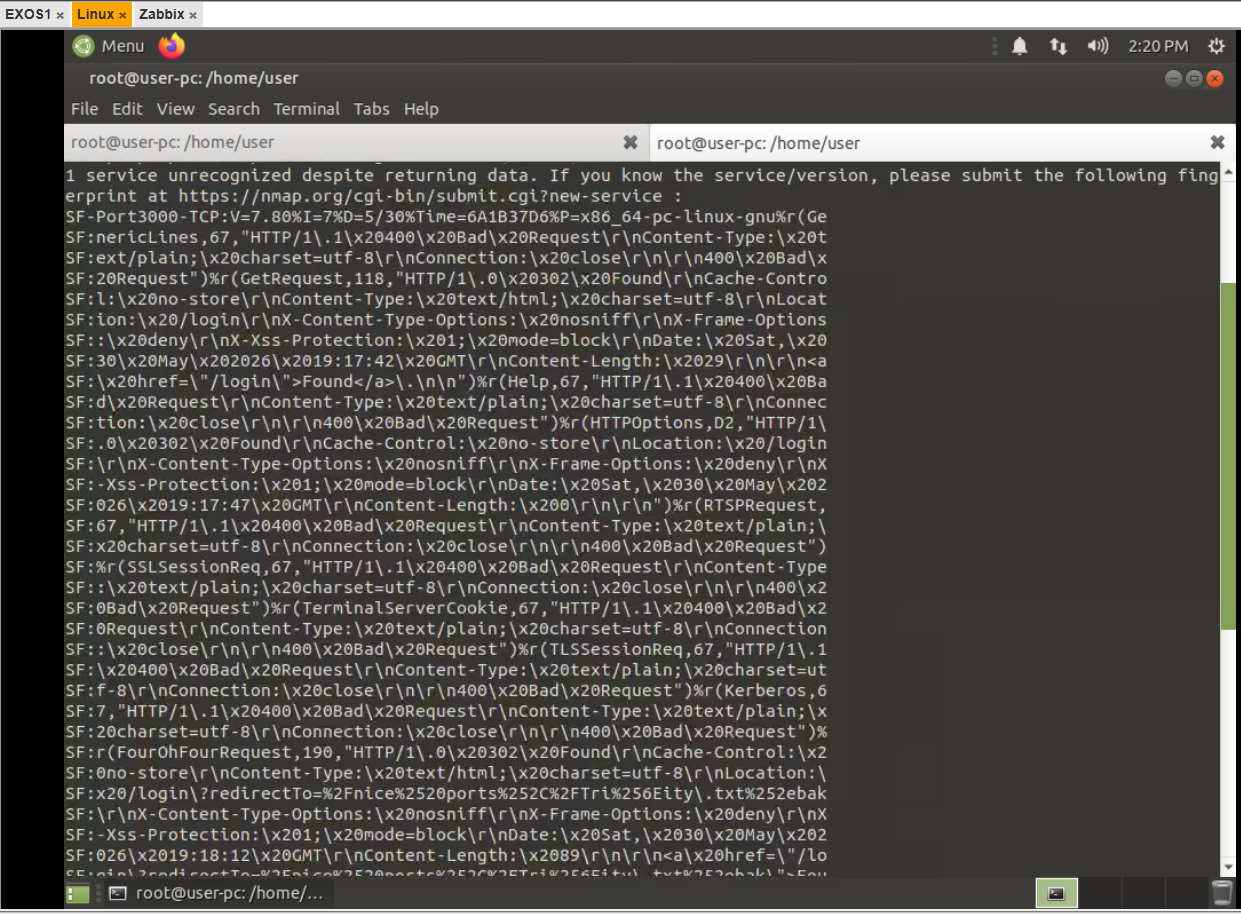
\includegraphics[width=1\linewidth]{fig/nmap6.png}
    \caption{Resultado da varredura utilizando o Nmap 2}
    \label{fig:nmap6}
\end{figure}

\begin{figure}[H]
    \centering
    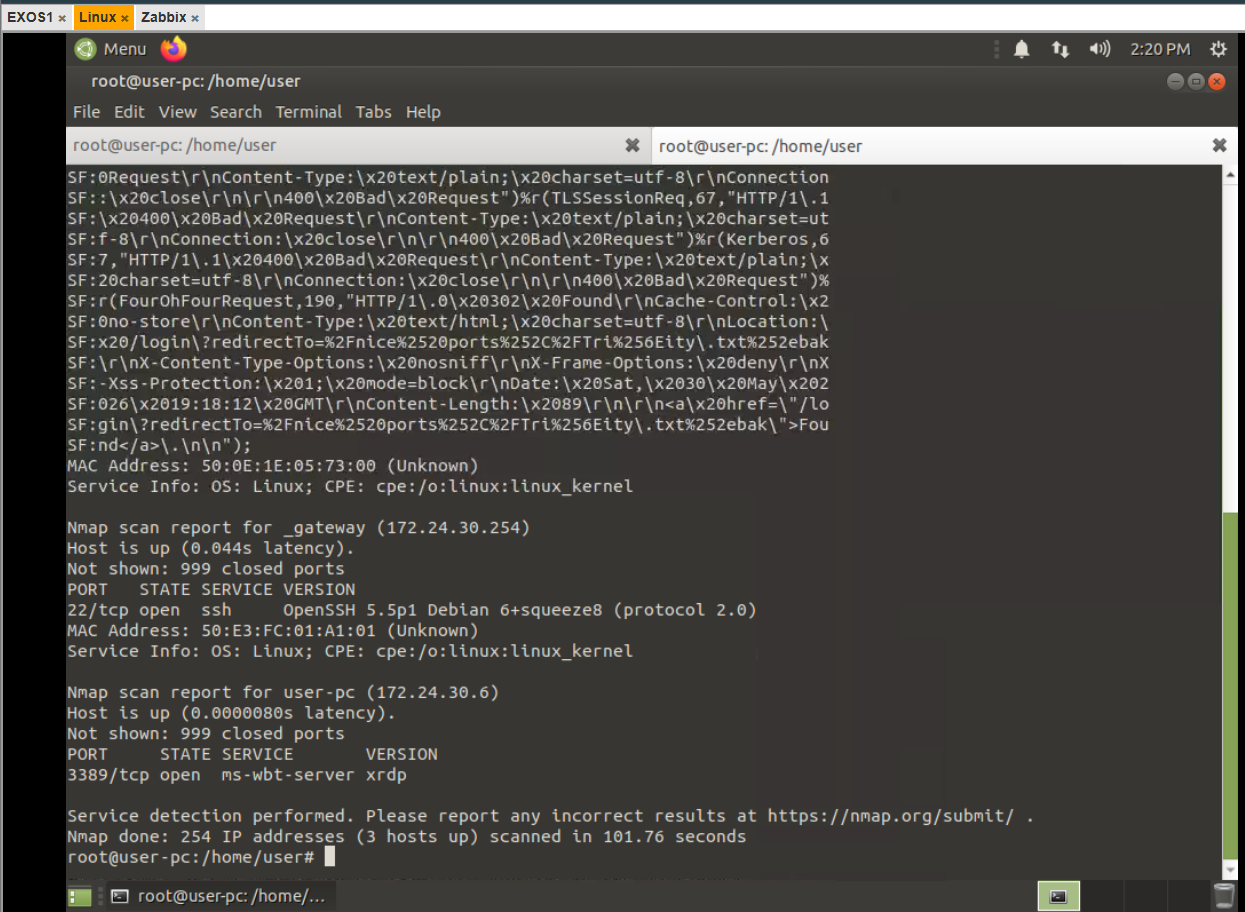
\includegraphics[width=1\linewidth]{fig/nmap7.png}
    \caption{Resultado da varredura utilizando o Nmap 3}
    \label{fig:nmap7}
\end{figure}

Como última simulação, foi utilizado o comando \textit{nmap 172.24.30.254 -A}. Por meio desse comando, é possível 
detectar o SO, a versão, verificar scripts e traceroute. Como resultado da varredura, 
foi possível identificar o sistema operacional do gateway, a versão do serviço SSH,
 bem como a presença de scripts de segurança e o caminho de rede para o host alvo.

\begin{figure}[H]
    \centering
    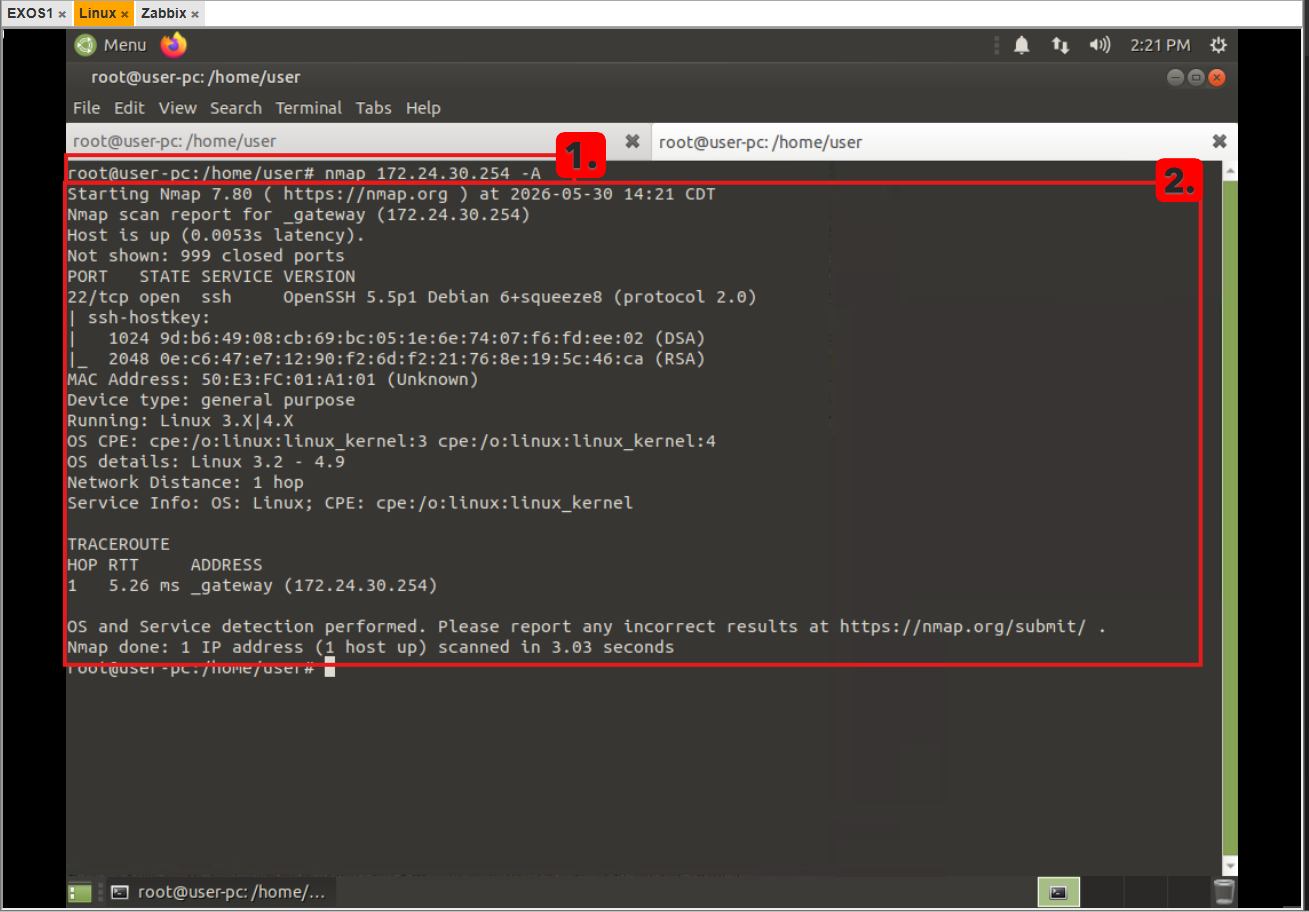
\includegraphics[width=1\linewidth]{fig/nmap8.png}
    \caption{Resultado da varredura utilizando o Nmap com a opção -A; 
    1. Comando para realizar a varredura de portas e identificação do tipo de serviços utilizando a opção -A; 
    2. Resultado da varredura indicando o sistema operacional, a versão do serviço SSH}
    \label{fig:nmap8}
\end{figure}

\subsection{UFW}


Para a primeira simulação, foi utilizado o comando \textit{ufw allow ssh}, 
mostrado na Figura \ref{fig:ufw1}, 
para permitir conexões SSH utilizando o UFW.
 O resultado do comando indicou que a regra foi adicionada com sucesso. Em seguida, foi utilizado
  o comando \textit{ufw status} para verificar o status do UFW,
  confirmando que a regra de permissão para conexões SSH estava ativa.
\begin{figure}[H]
    \centering
    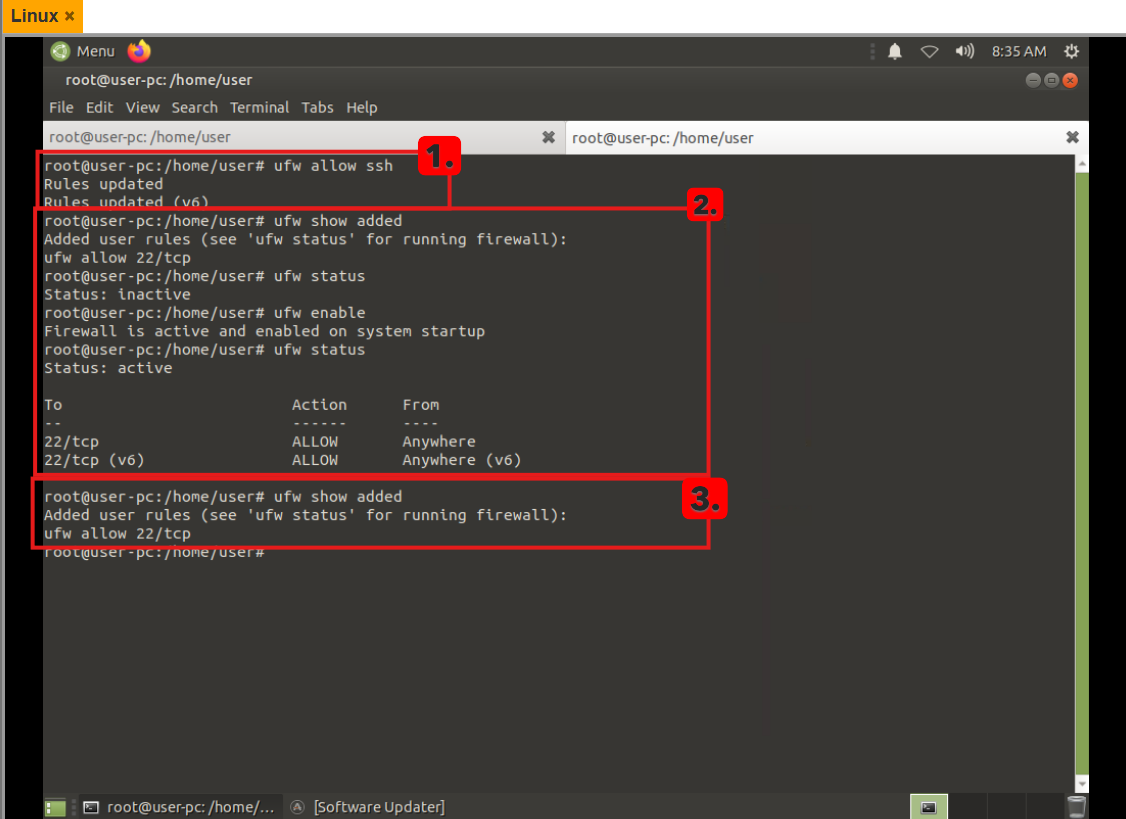
\includegraphics[width=1\linewidth]{fig/ufw1.png}
    \caption{Permitindo conexões SSH utilizando o UFW; 
    1. Comando para permitir conexões SSH; 
    2. Resultado do comando indicando que a regra foi adicionada com sucesso; 
    3. Comando para verificar o status do UFW;}
    \label{fig:ufw1}
\end{figure}

Na Figura \ref{fig:ufw2}, 
é possível observar o resultado do teste de conexão SSH entre o 
Host Linux e o Roteador ROT-ACME,
 indicando que a conexão foi estabelecida com sucesso, confirmando que a regra de permissão para
  conexões SSH estava funcionando corretamente.

\begin{figure}[H]
    \centering
    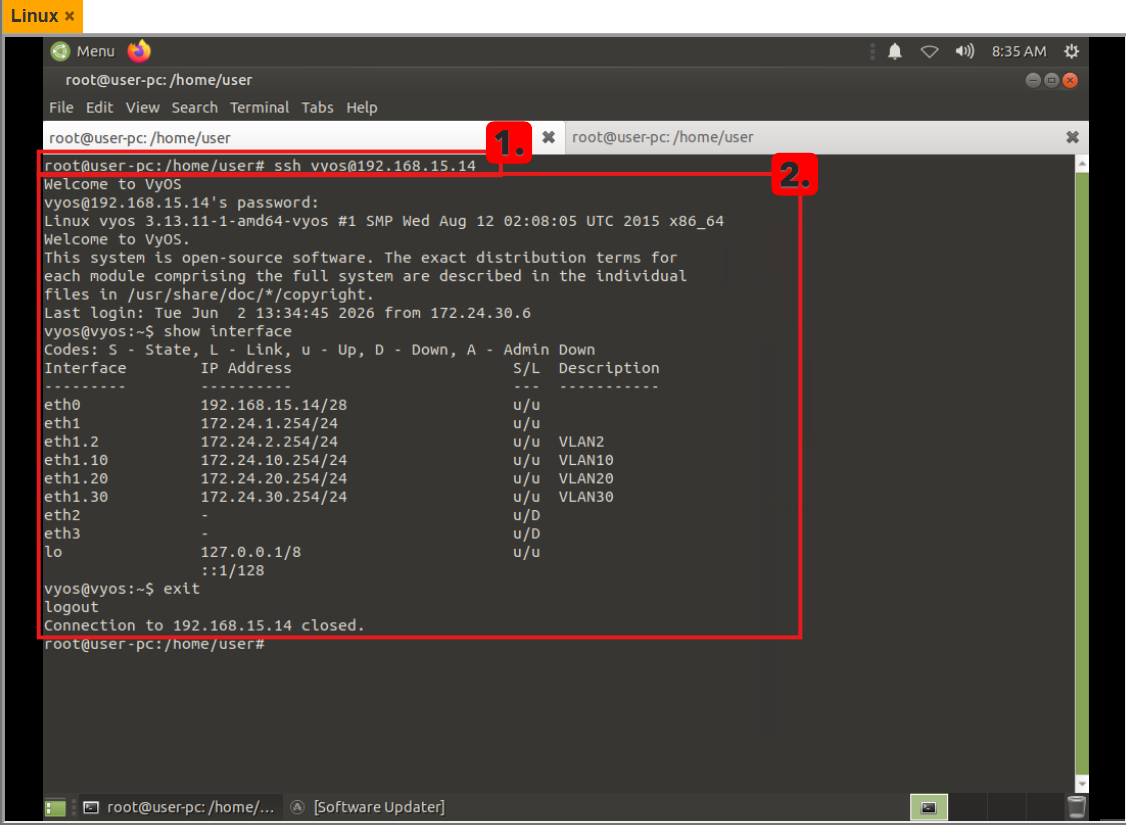
\includegraphics[width=1\linewidth]{fig/ufw2.png}
    \caption{Conexão SSH permitida utilizando o UFW; 
    1. Comando para realizar o SSH para o Roteador ROT-ACME;
    2. Resultado do comando indicando que a conexão SSH foi estabelecida com sucesso}
    \label{fig:ufw2}
\end{figure}

Em seguida, por meio do comando \textit{ufw deny ssh}, 
mostrado na Figura \ref{fig:ufw3},
 foi possível desabilitar o SSH utilizando o UFW. O resultado do comando 
 indicou que a regra de bloqueio para conexões SSH foi adicionada com sucesso. 
 Em seguida, foi utilizado o comando \textit{ufw status} para verificar o status do UFW, 
 confirmando que a regra de bloqueio para conexões SSH estava ativa.

\begin{figure}[H]
    \centering
    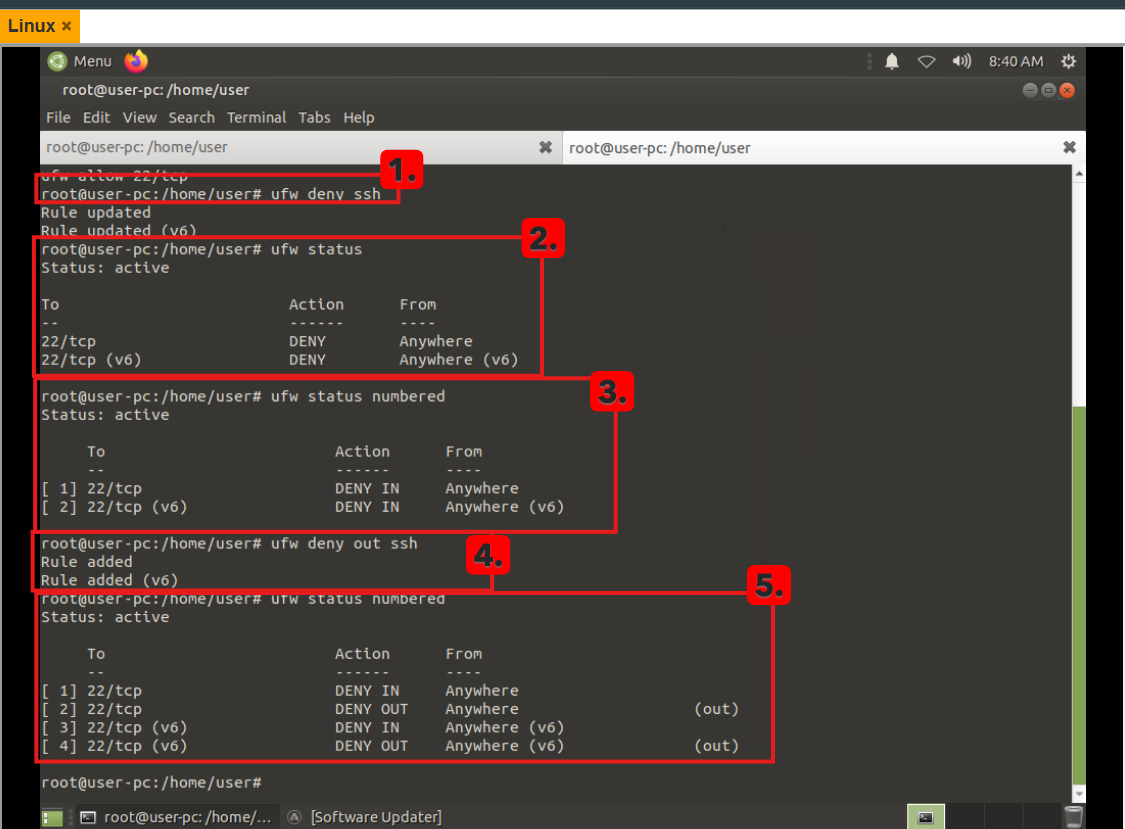
\includegraphics[width=1\linewidth]{fig/ufw3.png}
    \caption{Desabilitando o SSH utilizando o UFW;
     1. Comando para desabilitar o SSH para o Host Linux; 
     2. Resultado do comando indicando que a regra foi adicionada com sucesso;
     3. Comando para verificar o status do UFW enumerando as regras ativas;
     4. Comando para desabilitar o SSH do Host Linux para outros hosts utilizando o UFW;
     5. Resultado do comando indicando que a regra foi adicionada com sucesso;}
    \label{fig:ufw3}
\end{figure}

A Figura \ref{fig:ufw4} mostra o resultado do teste de
conexão SSH entre o Host Linux e o Roteador ROT-ACME, indicando que a conexão foi bloqueada 
com sucesso, confirmando que a regra de bloqueio para conexões SSH estava funcionando corretamente.

\begin{figure}[H]
    \centering
    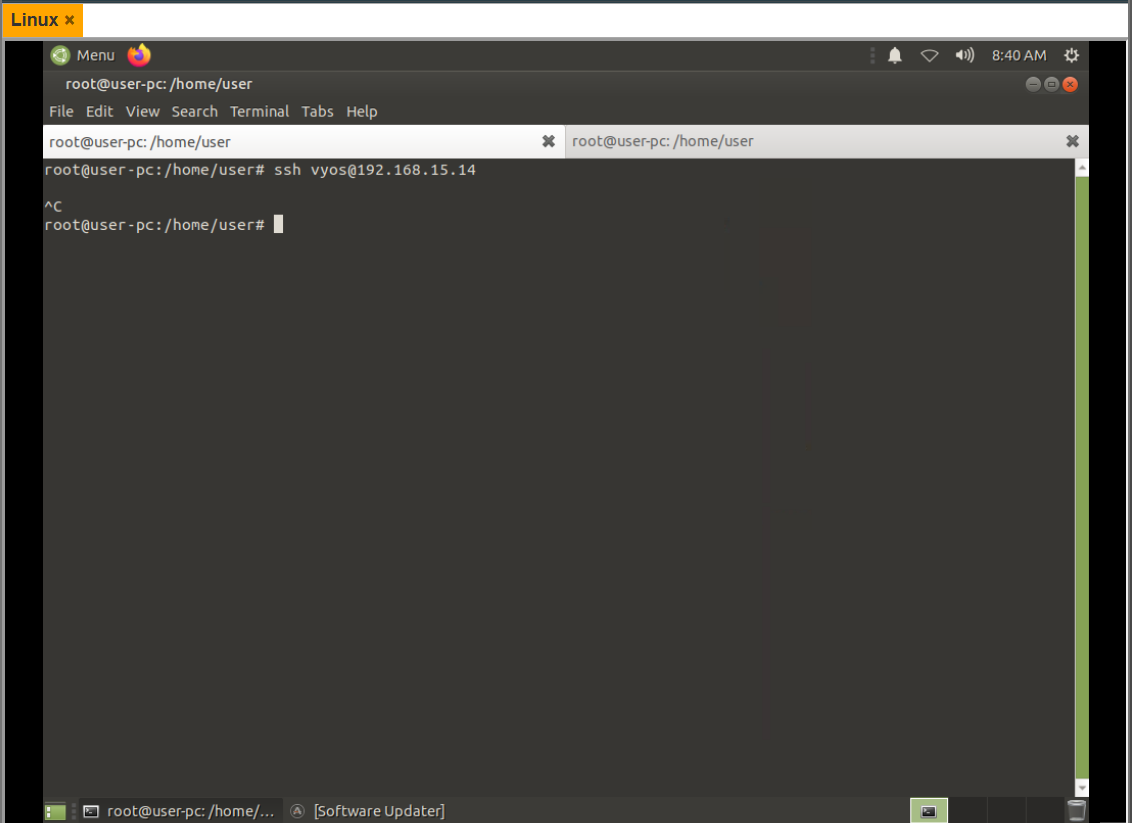
\includegraphics[width=1\linewidth]{fig/ufw4.png}
    \caption{Resultado do bloqueio do SSH utilizando o UFW;}
    \label{fig:ufw4}
\end{figure}

Na terceira simulação, foi utilizado o comando 
\textit{ufw delete deny ssh}, mostrado na Figura \ref{fig:ufw5}, para deletar a regra de 
bloqueio do SSH utilizando o UFW. O resultado do comando indicou que a regra foi deletada 
com sucesso. Em seguida, foi utilizado o comando \textit{ufw status}.       

\begin{figure}[H]
    \centering
    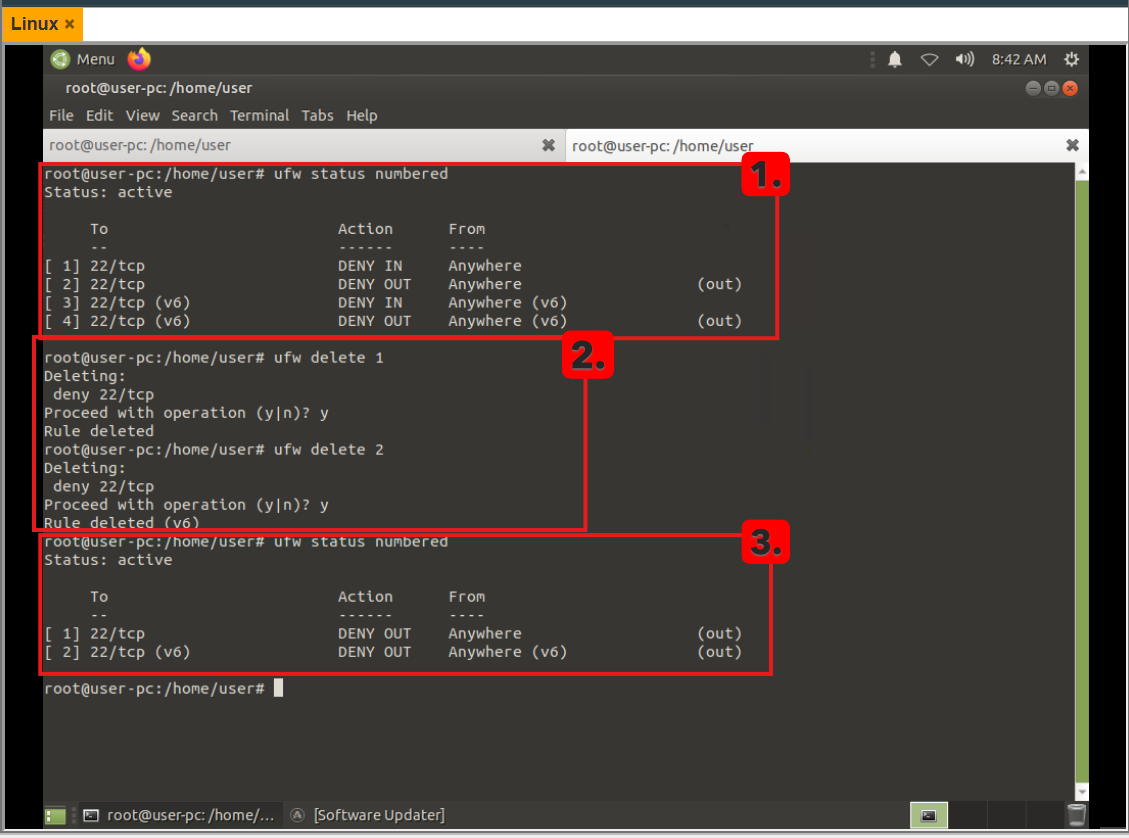
\includegraphics[width=1\linewidth]{fig/ufw5.png}
    \caption{Exclusão de uma regra no UFW;
    1. Comando para mostrar as regras ativas do UFW enumerando as regras;
    2. Comando para deletar a regra de bloqueio do SSH utilizando o número da regra;
    3. Resultado do comando indicando que a regra foi deletada com sucesso;}
    \label{fig:ufw5}
\end{figure}

Para visualizar a lista de serviços ativos, 
foi utilizado o comando \textit{ufw status}, mostrado na Figura \ref{fig:ufw6}.
 O resultado do comando indicou que a regra de permissão para conexões SSH estava ativa. 
 Em seguida, foi utilizado o comando \textit{ufw disable} para desabilitar o UFW,
  e o resultado do comando indicou que o firewall foi desabilitado com sucesso.

\begin{figure}[H]
    \centering
    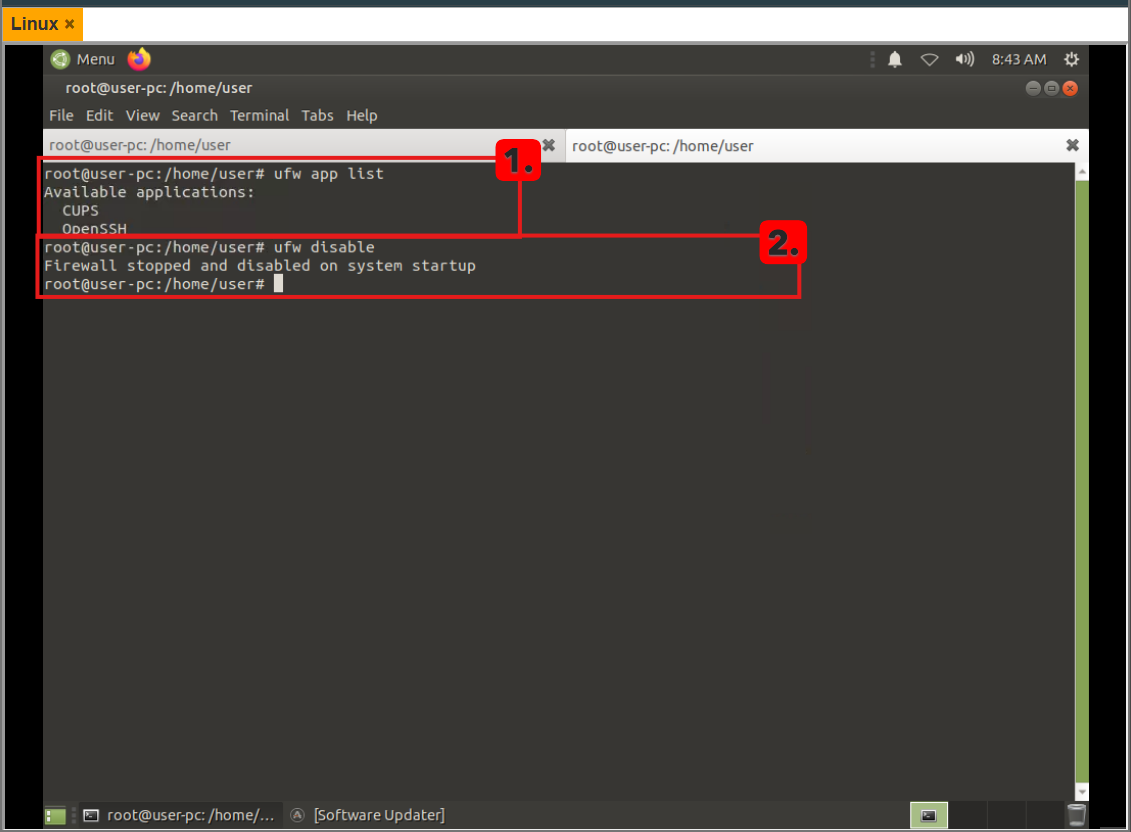
\includegraphics[width=1\linewidth]{fig/ufw6.png}
    \caption{1. Comando para visualizar a lista de serviços ativos;
    2. Comando para desabilitar o UFW;}
    \label{fig:ufw6}
\end{figure}

Já na última simulação, foi utilizado o comando \textit{ufw default enable deny incoming}, mostrado na 
Figura \ref{fig:ufw7}, para configurar a política padrão do UFW para negar conexões de entrada. 
O resultado do comando indicou que a política padrão para conexões de entrada foi 
configurada com sucesso. Em seguida, foi utilizado o comando \textit{ufw default allow outgoing} 
para configurar a política padrão do UFW para permitir conexões de saída,
 e o resultado do comando indicou que a política padrão para conexões de saída foi configurada com sucesso.

\begin{figure}[H]
    \centering
    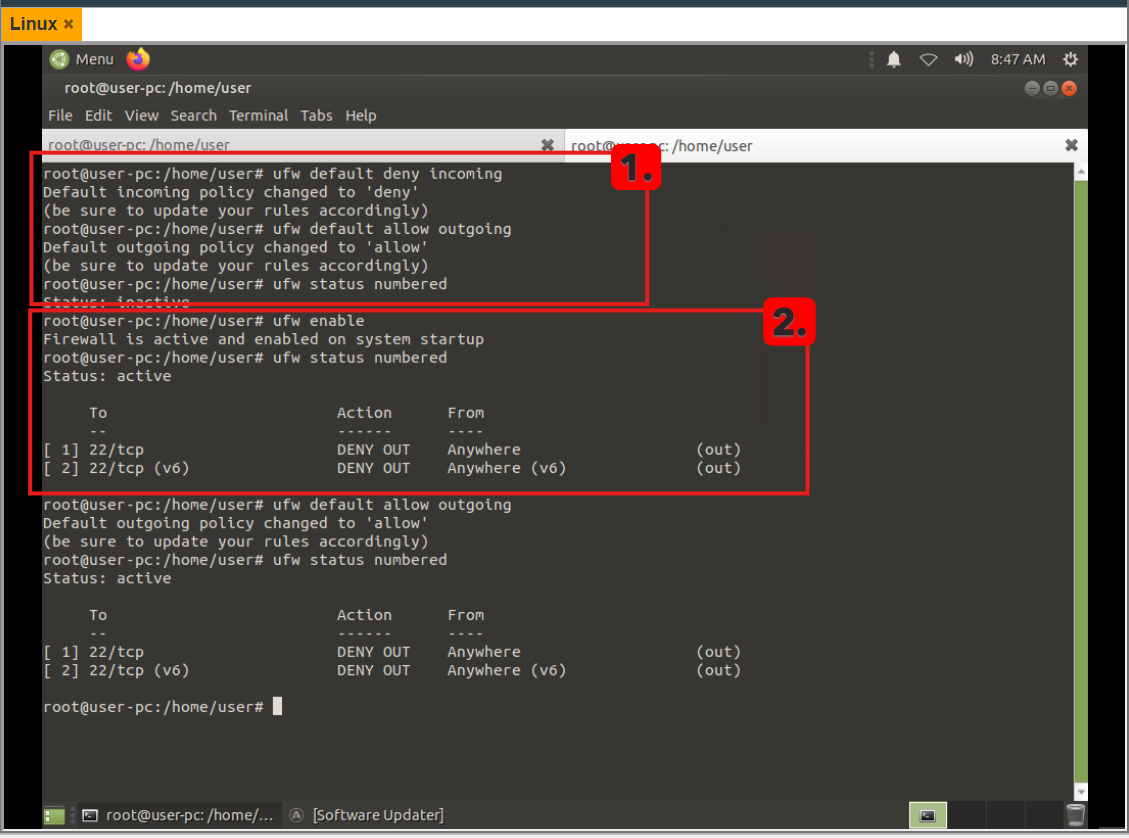
\includegraphics[width=1\linewidth]{fig/ufw7.png}
    \caption{1. Comando para bloquear política de entrada; 
    2. Comando para permitir política de saída;}
    \label{fig:ufw7}
\end{figure}

\subsection{SNORT}

Para as simulações com o Snort, inicialmente foi testado o envio de notificações no ambiente Linux
utilizando o comando \textit{notify-send}, como mostrado na Figura \ref{fig:snort1}. Esse teste foi
realizado para verificar se o sistema conseguia exibir alertas na interface gráfica, recurso utilizado
posteriormente para apresentar as notificações geradas a partir das detecções do Snort.

\begin{figure}[H]
    \centering
    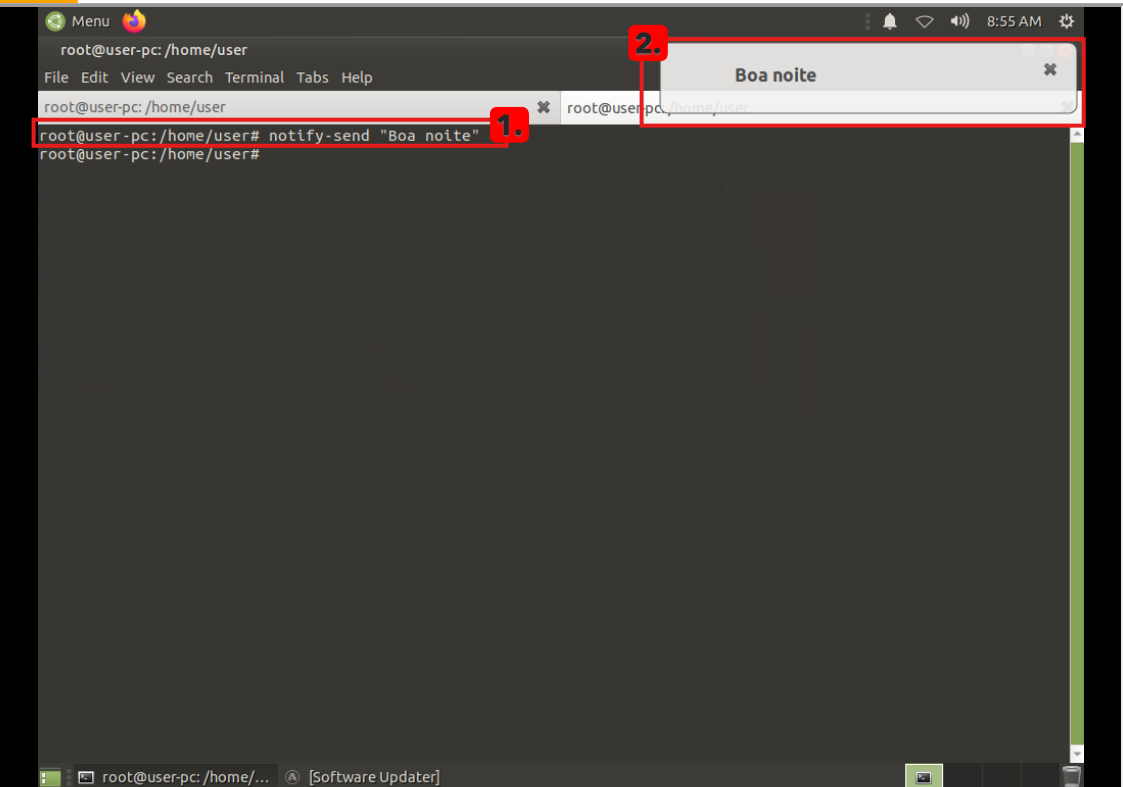
\includegraphics[width=1\linewidth]{fig/snort1.png}
    \caption{Notificação utilizando o notify-send;
     1. Comando notify-send para enviar uma notificação; 
     2. Resultado do comando indicando que a notificação foi enviada com sucesso}
    \label{fig:snort1}
\end{figure}


Em seguida, foi adicionada uma regra personalizada no arquivo \textit{/etc/snort/rules/local.rules},
conforme apresentado na Figura \ref{fig:snort2}. A regra configurada utiliza a ação \textit{alert}
para pacotes do tipo ICMP, permitindo que o Snort gere um alerta sempre que for identificado tráfego
de ping na rede. A mensagem definida para o alerta foi \textit{ECMP ECHO Request detectado}, com o
identificador \textit{sid: 1000001}.

\begin{figure}[H]
    \centering
    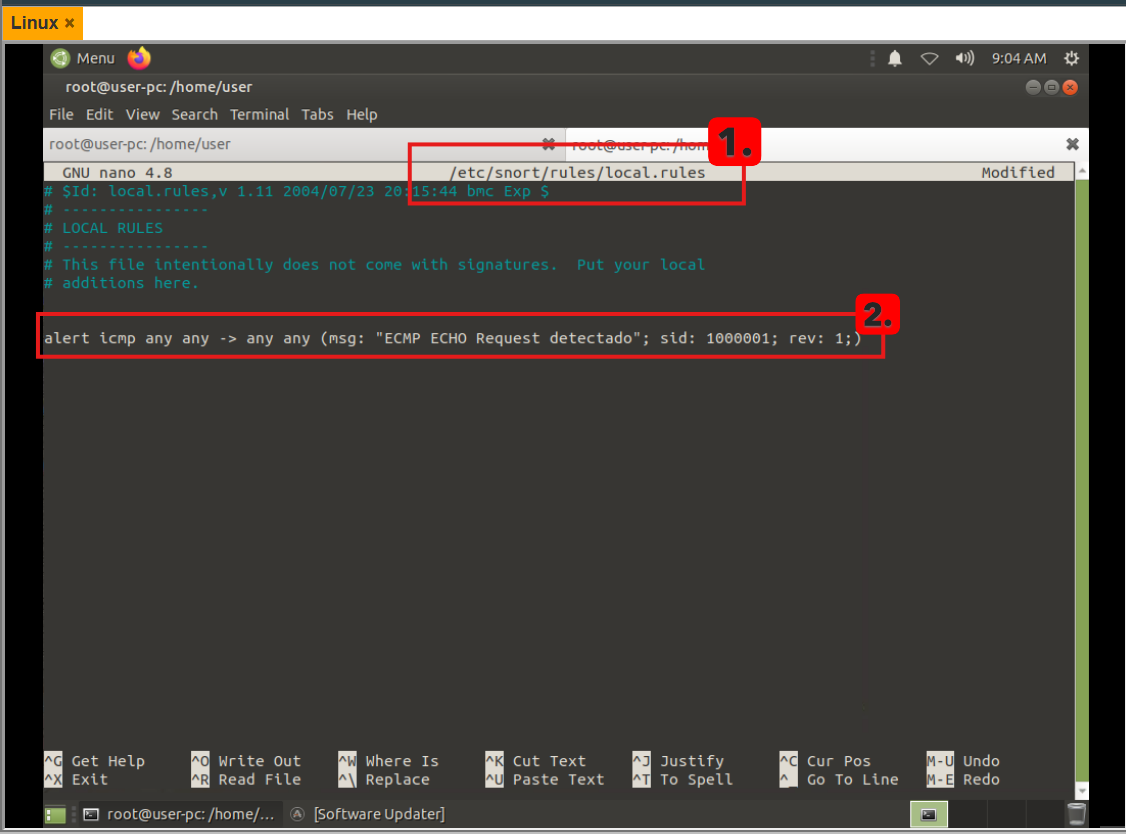
\includegraphics[width=1\linewidth]{fig/snort2.png}
    \caption{Adicionando uma regra personalizada no Snort;
     1. Caminho do arquivo de regras do Snort; 
     2. Regra personalizada para detectar tráfego ICMP;}
    \label{fig:snort2}
\end{figure}

Após a criação da regra, foi realizado um teste de conectividade com o comando \textit{ping 172.24.30.6},
partindo do LinuxDesktop para o Host Linux, como mostrado na Figura \ref{fig:snort4}. O teste gerou
pacotes ICMP Echo Request e Echo Reply, que serviram como tráfego de entrada para validar a regra
personalizada configurada no Snort.

\begin{figure}[H]
    \centering
    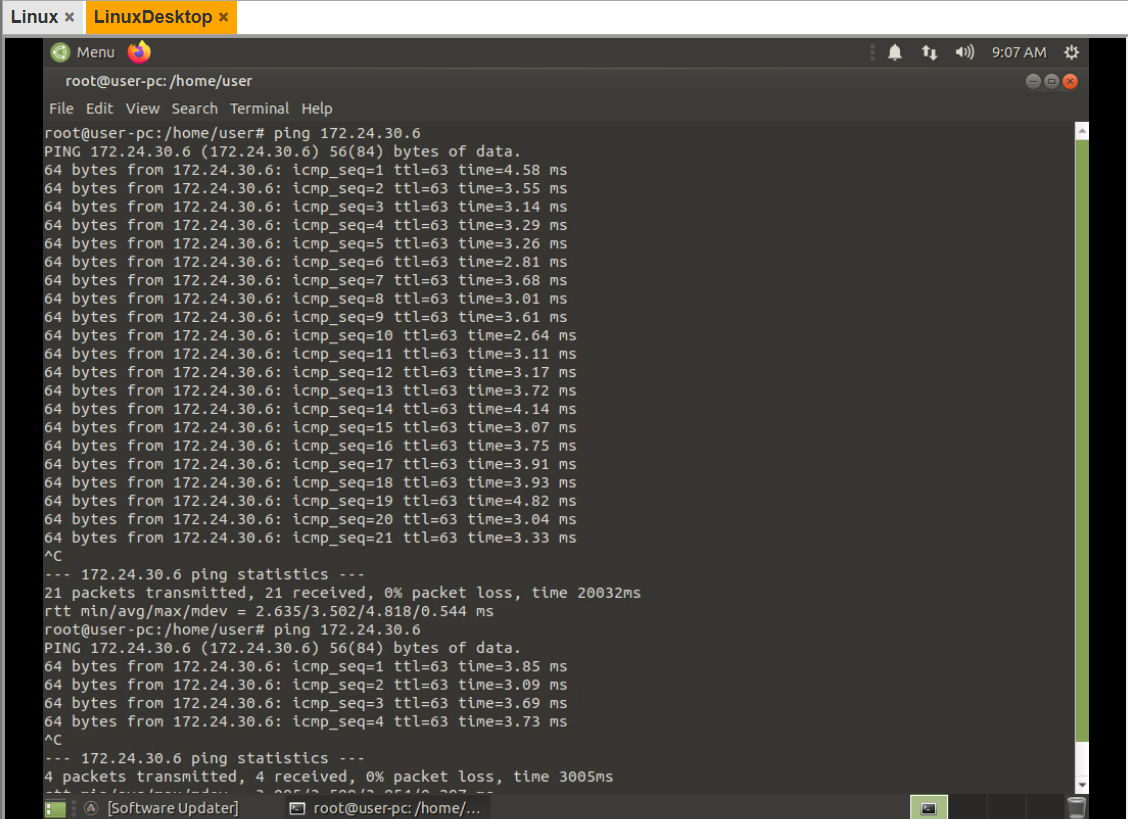
\includegraphics[width=1\linewidth]{fig/snort4.png}
    \caption{Ping realizado do LinuxDesktop para o Host Linux}
    \label{fig:snort4}
\end{figure}


Na Figura \ref{fig:snort3}, é possível observar a execução do Snort em modo console, utilizando o
arquivo de regras personalizado e a interface de rede \textit{ens3}. O comando
\textit{snort -A console -q -c /etc/snort/rules/local.rules -dev -i ens3} monitora os pacotes
capturados e exibe os alertas diretamente no terminal. Como resultado, o Snort identificou o tráfego
ICMP gerado pelo teste de ping e exibiu os alertas correspondentes, contendo os endereços IP de origem
e destino, o tipo ICMP e os dados do pacote.

\begin{figure}[H]
    \centering
    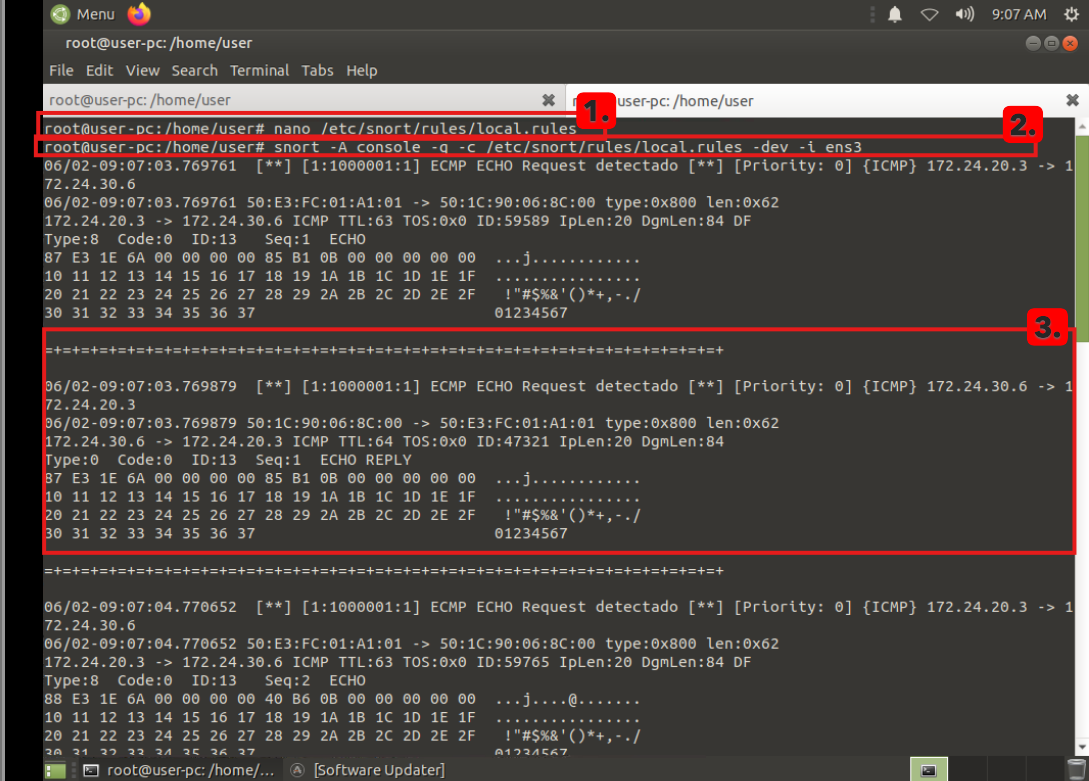
\includegraphics[width=1\linewidth]{fig/snort3.png}
    \caption{1. Comando para acessar o arquivo de regras do Snort;
    2. Execução do Snort para monitorar o tráfego de rede e detectar pacotes ICMP;
    3. Resultado do comando indicando que um pacote ICMP foi detectado
    }
    \label{fig:snort3}
\end{figure}



Na segunda simulação, o Snort foi executado novamente, porém redirecionando a saída para o arquivo
\textit{infoSnort.txt}, conforme mostrado na Figura \ref{fig:snort5}. Após a interrupção da captura,
foi utilizado o comando \textit{notify-send "\$(cat infoSnort.txt)"} para enviar o conteúdo do arquivo
como uma notificação do sistema. Dessa forma, os alertas detectados pelo Snort puderam ser visualizados
fora do terminal.

\begin{figure}[H]
    \centering
    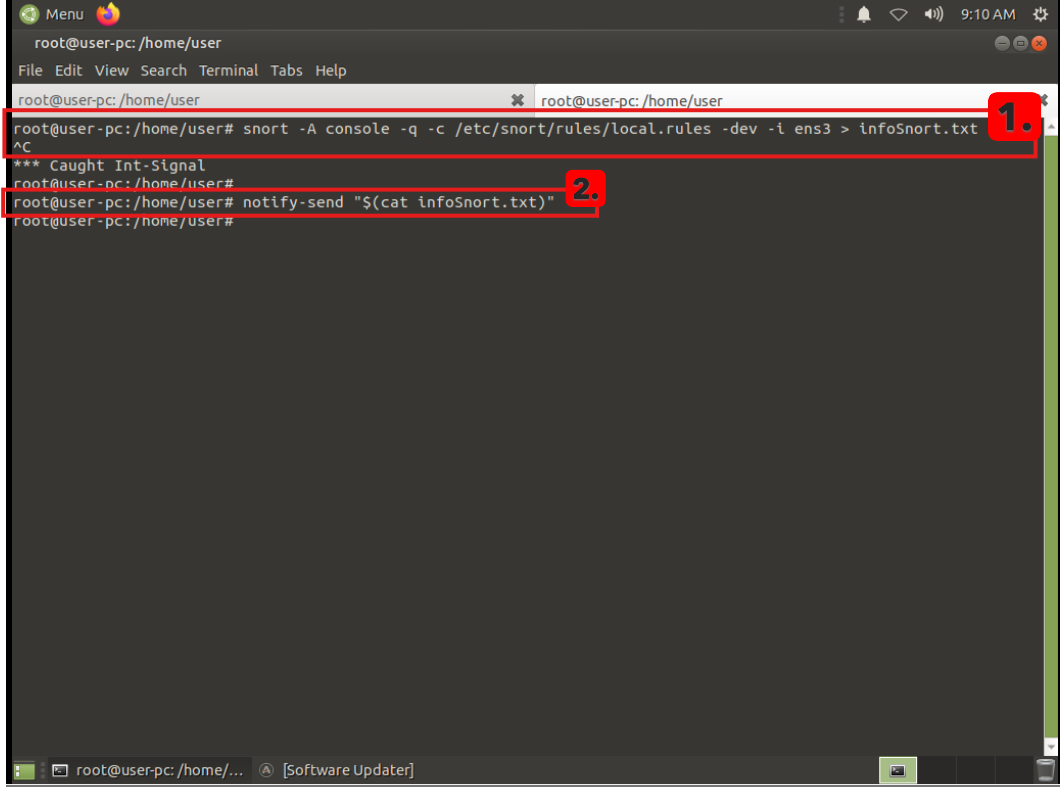
\includegraphics[width=1\linewidth]{fig/snort5.png}
    \caption{1. Comando para executar o snort no arquivo infoSnort.txt;
    2. Comando para visualizar o conteúdo do arquivo infoSnort.txt;}
    \label{fig:snort5}
\end{figure}

A Figura \ref{fig:snort6} apresenta o resultado da notificação gerada a partir do arquivo
\textit{infoSnort.txt}. Nela, é possível observar os alertas de detecção do tráfego ICMP, incluindo
requisições e respostas entre os hosts 172.24.20.3 e 172.24.30.6. Esse resultado confirma que a regra
personalizada foi acionada corretamente e que a saída do Snort pode ser reaproveitada para gerar
avisos visuais no sistema.

\begin{figure}[H]
    \centering
    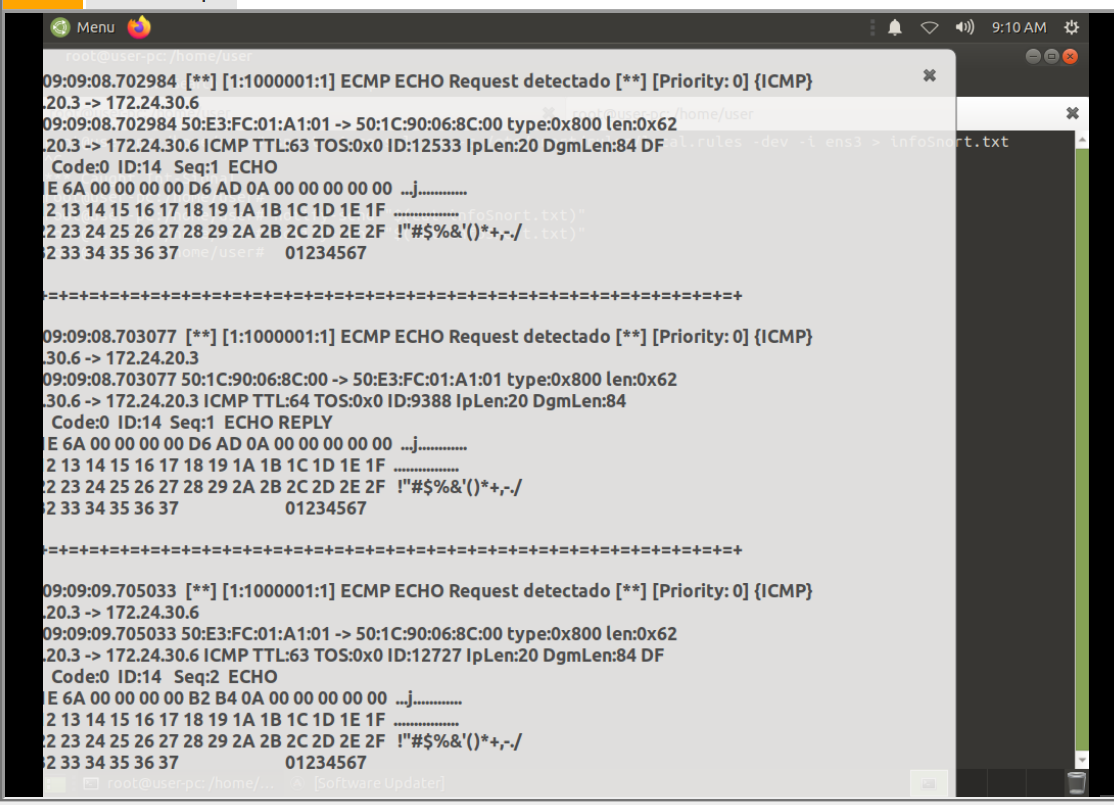
\includegraphics[width=1\linewidth]{fig/snort6.png}
    \caption{Resultado do arquivo infoSnort.txt indicando a detecção de um pacote ICMP.}
    \label{fig:snort6}
\end{figure}

Também foi configurada a saída de alertas do Snort no arquivo \textit{/etc/snort/snort.conf}, como
mostrado na Figura \ref{fig:snort7}. Nessa etapa, foi adicionada a diretiva
\textit{output alert\_fast: alert.fast}, responsável por armazenar os alertas gerados pelo Snort no
formato rápido, facilitando a leitura e o acompanhamento dos eventos detectados.

\begin{figure}[H]
    \centering
    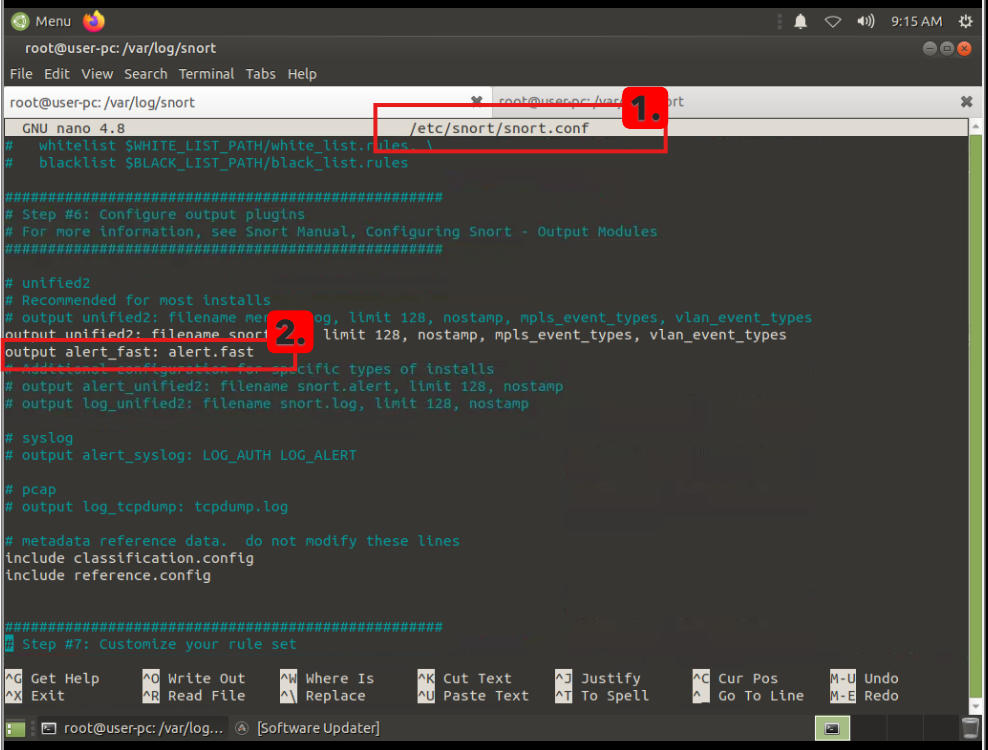
\includegraphics[width=1\linewidth]{fig/snort7.png}
    \caption{Adicionando na configuração do Snort o arquivo que será 
    utilizado para armazenar os alertas gerados pelo Snort;}
    \label{fig:snort7}
\end{figure}

Por fim, para automatizar o processo de monitoramento dos alertas do Snort, 
foram criadas regras personalizadas no arquivo \textit{/etc/snort/rules/local.rules}, como mostrado na Figura \ref{fig:snort8}. 
Essas regras foram configuradas para detectar tráfego de rede relacionado a protocolos como ICMP,
 SSH, HTTP e HTTPS. Com essas regras em vigor, o Snort será capaz de identificar e gerar alertas sempre que
  for detectado tráfego suspeito ou malicioso relacionado a esses protocolos, 
  permitindo uma resposta mais rápida e eficaz a potenciais ameaças na rede.    

\begin{figure}[H]
    \centering
    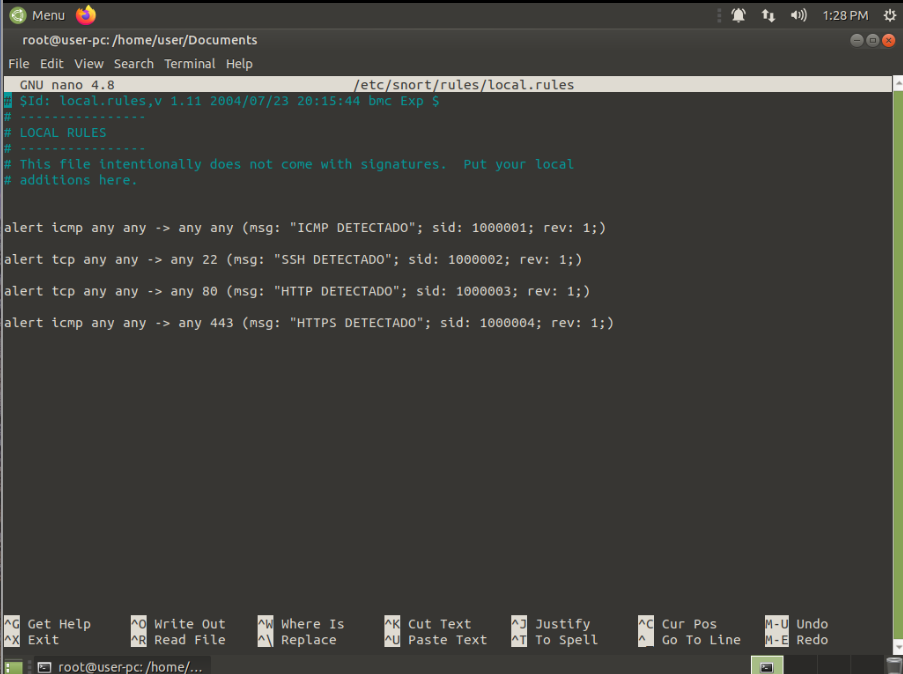
\includegraphics[width=1\linewidth]{fig/snort8.png}
    \caption{Adição de novas regras personalizadas no arquivo local.rules para detectar tráfego ICMP, SSH, HTTP e HTTPS.}
    \label{fig:snort8}
\end{figure}

Na Figura \ref{fig:snort9}, é possível observar a ativação e inicialização do serviço
\textit{snort-monitor} por meio dos comandos \textit{systemctl enable snort-monitor} e
\textit{systemctl start snort-monitor}. Em seguida, o comando \textit{systemctl status snort-monitor}
confirmou que o serviço estava ativo e em execução, indicando que o monitoramento de alertas do Snort
foi configurado corretamente.

\begin{figure}[H]
    \centering
    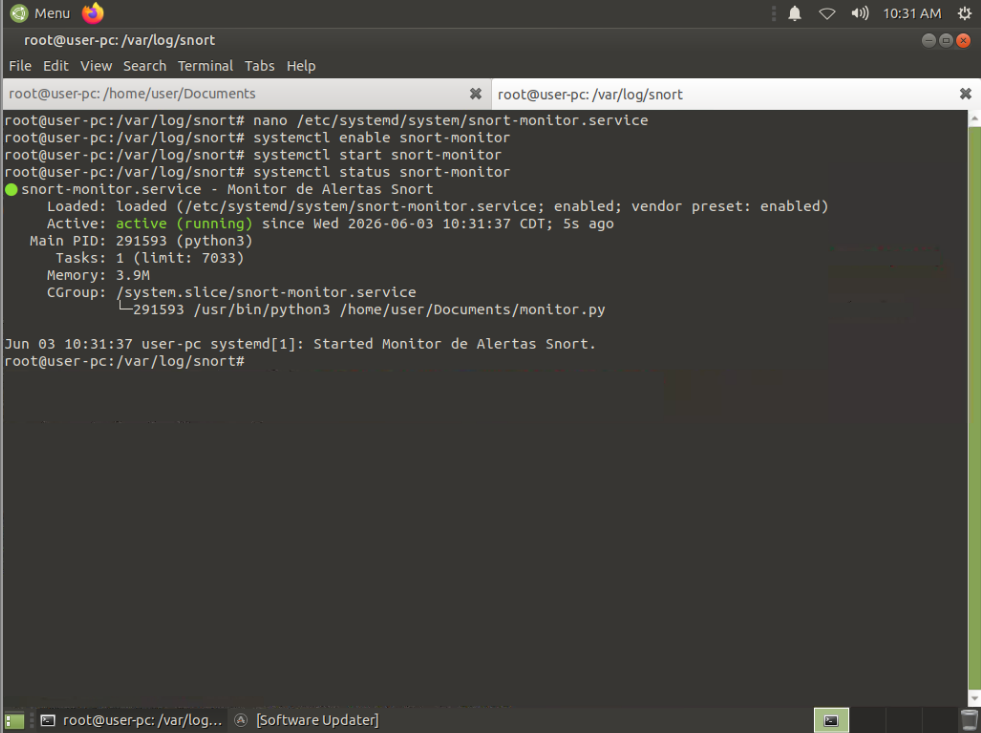
\includegraphics[width=1\linewidth]{fig/snort9.png}
    \caption{Inicialização do serviço snort-monitor;
    1. Comandos para habilitar, iniciar e verificar o status do serviço;
    2. Resultado indicando que o serviço está ativo e em execução}
    \label{fig:snort9}
\end{figure}

Foi criado o arquivo monitor.py \ref{lst:monitor} para monitorar o arquivo de alertas do Snort e 
enviar notificações utilizando o notify-send. O script lê o conteúdo do arquivo de alertas,
 verifica se há novas entradas e envia uma notificação para cada novo alerta detectado.
  O script foi configurado para ser executado periodicamente, garantindo que as notificações 
  sejam enviadas em tempo real sempre que um novo alerta for gerado pelo Snort.

Na Figura \ref{fig:snort10}, foi feita a configuração do script monitor.py para ser executado
utilizando a interface \textit{Startup Program}, que executa o arquivo monitor.py automaticamente
 durante a inicialização do sistema. Dessa forma, 
 o monitoramento dos alertas do Snort e o envio de notificações estarão ativos desde o momento em que o 
 sistema for iniciado, garantindo uma resposta imediata a qualquer evento detectado pelo Snort.

\begin{figure}[H]
    \centering
    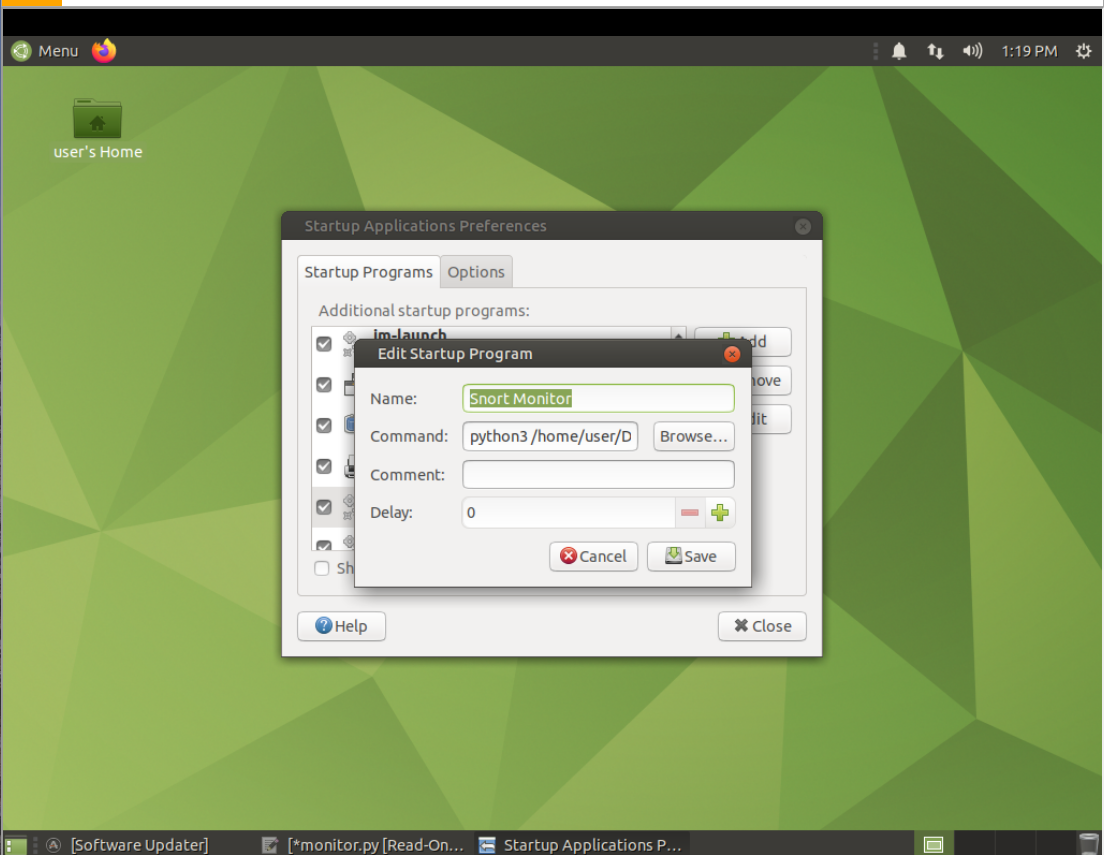
\includegraphics[width=1\linewidth]{fig/snort10.png}
    \caption{Configuração do monitor.py para inicialização automática pelo Startup Program}
    \label{fig:snort10}
\end{figure}

Já na Figura \ref{fig:snort11}, é possível observar o resultado do monitoramento do arquivo de alertas do Snort,
onde cada nova entrada no arquivo de alertas gera uma notificação utilizando o notify-send. As notificações exibem 
o conteúdo dos alertas, permitindo que o usuário seja informado em tempo real.


\begin{figure}[H]
    \centering
    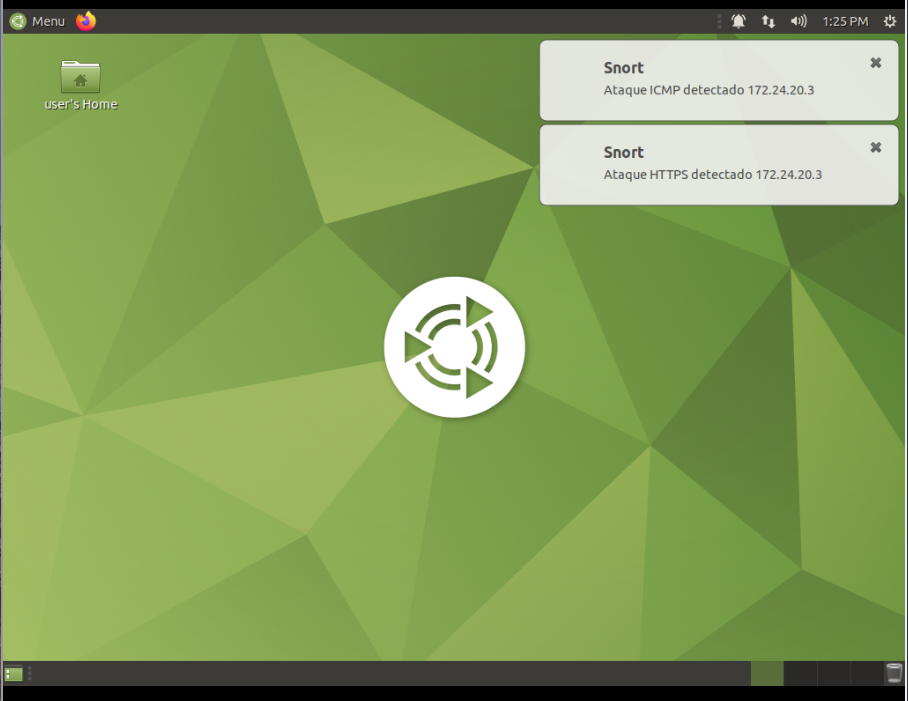
\includegraphics[width=1\linewidth]{fig/snort11.png}
    \caption{Notificações geradas a partir do monitoramento dos alertas do Snort}
    \label{fig:snort11}
\end{figure}



\section{Conclusão}

Com a realização deste trabalho, foi possível analisar diferentes ferramentas utilizadas no gerenciamento, teste e segurança de redes. As simulações com o Iperf3 permitiram avaliar a largura de banda entre os hosts e verificar o comportamento da rede durante a transmissão de tráfego TCP e UDP, representando cenários de transferência de arquivos e comunicação de voz. Dessa forma, foi possível observar a capacidade da infraestrutura em manter a comunicação entre os dispositivos de forma estável.

O Nmap foi utilizado para realizar varreduras de portas, identificar serviços ativos e obter informações sobre os hosts presentes na rede. A partir dos testes, foi possível reconhecer quais portas estavam abertas, quais serviços estavam disponíveis e como diferentes tipos de varredura auxiliam no diagnóstico e na análise de segurança da infraestrutura.

Com o UFW, foram aplicadas regras de firewall para permitir, bloquear e remover permissões de acesso, principalmente relacionadas ao serviço SSH. Esses testes demonstraram a importância do controle de tráfego por meio de regras simples e objetivas, permitindo validar na prática o funcionamento do bloqueio e da liberação de conexões.

Por fim, o Snort foi utilizado para detectar tráfego ICMP e gerar alertas a partir de regras personalizadas. A integração dos alertas com notificações do sistema mostrou como uma ferramenta de detecção de intrusão pode auxiliar no monitoramento da rede em tempo real. Assim, o conjunto de ferramentas estudado contribuiu para compreender melhor o desempenho, a identificação de serviços, o controle de acesso e a detecção de eventos em uma rede de computadores.


%-------------------------------------------------------------------------

{\small
\bibliography{egbib}
\bibliographystyle{ieee_fullname}
}

%-------------------------------------------------------------------------
\clearpage
\onecolumn

\appendices

\section{Configuração do Roteador ROT-ACME}

\begin{listing}[H]
\centering
\begin{minted}[
    bgcolor=bgcolor,
    frame=lines,
    breaklines=true,
    breakanywhere=true,
    fontsize=\footnotesize,
]{bash}

vyos@vyos:~$ configure

vyos@vyos:~# set interfaces ethernet eth0 address 172.24.254.2/30
vyos@vyos:~# set interfaces ethernet eth1 address 172.24.1.254/24 

vyos@vyos:~# set interfaces ethernet eth1 vif 20 description 'INTRANET'
vyos@vyos:~# set interfaces ethernet eth1 vif 20 address '172.24.20.254/24'
vyos@vyos:~# set interfaces ethernet eth1 vif 30 description 'DC'
vyos@vyos:~# set interfaces ethernet eth1 vif 30 address '172.24.30.254/24'

vyos@vyos:~# set protocols static route 0.0.0.0/0 next-hop 172.24.254.1

vyos@vyos:~# set service dhcp-server shared-network-name INTRANET subnet 172.24.20.0/24 default-router '172.24.20.254'
vyos@vyos:~# set service dhcp-server shared-network-name INTRANET subnet 172.24.20.0/24 dns-server '172.16.30.11'
vyos@vyos:~# set service dhcp-server shared-network-name INTRANET subnet 172.24.20.0/24 start '172.24.20.10' stop '172.24.20.100'

vyos@vyos:~# set service dhcp-server shared-network-name DC subnet 172.24.30.0/24 default-router '172.24.30.254'
vyos@vyos:~# set service dhcp-server shared-network-name DC subnet 172.24.30.0/24 dns-server '172.16.30.11'
vyos@vyos:~# set service dhcp-server shared-network-name DC subnet 172.24.30.0/24 start '172.24.30.10' stop '172.24.30.100'

vyos@vyos:~# set service snmp community grs authorization rw
vyos@vyos:~# set service snmp community grs network 172.24.0.0/16
vyos@vyos:~# set service snmp community grs client 172.24.1.254
vyos@vyos:~# set service snmp trap-target 172.24.1.254 community grs

vyos@vyos:~# commit
vyos@vyos:~# save
vyos@vyos:~# exit 

\end{minted}
\caption{Configuração de Roteador ROT-ACME}
\label{lst:rotacme}
\end{listing}


\section{Configuração do Roteador R1}

O Código \ref{lst:rotR1} apresenta a configuração realizada no roteador R1 utilizando o sistema operacional VyOS. A configuração contempla endereçamento IP, NAT, protocolo OSPF e monitoramento via SNMP.

\begin{listing}[H]
\centering
\begin{minted}[
    bgcolor=bgcolor,
    frame=lines,
    breaklines=true,
    breakanywhere=true,
    fontsize=\footnotesize,
]{bash}

vyos@vyos:~$ configure
vyos@vyos:~# set interfaces ethernet eth0 address dhcp
vyos@vyos:~# set interfaces ethernet eth1 address 192.168.15.17/28
vyos@vyos:~# set interfaces ethernet eth2 address 192.168.15.33/28
vyos@vyos:~# set interfaces loopback lo address 10.1.1.1/32

vyos@vyos:~# set nat source rule 100 outbound-interface 'eth0'
vyos@vyos:~# set nat source rule 100 source address '192.168.15.0/24'
vyos@vyos:~# set nat source rule 100 translation address 'masquerade'

vyos@vyos:~# set protocols ospf area 0 network 192.168.122.0/24
vyos@vyos:~# set protocols ospf area 0 network 192.168.15.16/28
vyos@vyos:~# set protocols ospf area 0 network 192.168.15.32/28

vyos@vyos:~# set protocols ospf default-information originate 
vyos@vyos:~# set protocols ospf default-information originate metric 10
vyos@vyos:~# set protocols ospf default-information originate metric-type 2

vyos@vyos:~# set protocols ospf log-adjacency-changes
vyos@vyos:~# set protocols ospf parameters router-id 10.1.1.1
vyos@vyos:~# set protocols ospf redistribute connected metric-type 2
vyos@vyos:~# set protocols ospf redistribute connected route-map CONNECT

vyos@vyos:~# set policy route-map CONNECT rule 10 action permit
vyos@vyos:~# set policy route-map CONNECT rule 10 match interface lo

vyos@vyos:~# set service snmp community grs authorization rw
vyos@vyos:~# set service snmp community grs network 192.168.15.0/24
vyos@vyos:~# set service snmp community grs client 192.168.15.33
vyos@vyos:~# set service snmp trap-target 192.168.15.33 community grs

vyos@vyos:~# commit
vyos@vyos:~# save
vyos@vyos:~# exit

\end{minted}
\caption{Configuração do roteador R1 em VyOS}
\label{lst:rotR1}
\end{listing}

\section{Configuração do Roteador R2}

\begin{listing}[H]
\centering
\begin{minted}[
    bgcolor=bgcolor,
    frame=lines,
    breaklines=true,
    breakanywhere=true,
    fontsize=\footnotesize,
]{bash}

vyos@vyos:~$ configure

vyos@vyos:~# set interfaces ethernet eth0 address dhcp
vyos@vyos:~# set interfaces ethernet eth1 address 192.168.15.18/28
vyos@vyos:~# set interfaces ethernet eth2 address 192.168.15.35/28
vyos@vyos:~# set interfaces ethernet eth3 address 192.168.15.50/28
vyos@vyos:~# set interfaces loopback lo address 10.2.2.2/32

vyos@vyos:~# set nat source rule 100 outbound-interface name 'eth0'
vyos@vyos:~# set nat source rule 100 source address '192.168.15.0/24'
vyos@vyos:~# set nat source rule 100 translation address 'masquerade'

vyos@vyos:~# set protocols ospf area 0 network 192.168.15.0/28
vyos@vyos:~# set protocols ospf area 0 network 192.168.15.16/28
vyos@vyos:~# set protocols ospf area 0 network 192.168.15.32/28
vyos@vyos:~# set protocols ospf area 0 network 192.168.15.48/28

vyos@vyos:~# set protocols ospf default-information originate
vyos@vyos:~# set protocols ospf default-information originate metric 100
vyos@vyos:~# set protocols ospf default-information originate metric-type 2

vyos@vyos:~# set protocols ospf log-adjacency-changes
vyos@vyos:~# set protocols ospf parameters router-id 10.2.2.2
vyos@vyos:~# set protocols ospf redistribute connected metric-type 2
vyos@vyos:~# set protocols ospf redistribute connected route-map CONNECT

vyos@vyos:~# set policy route-map CONNECT rule 10 action permit
vyos@vyos:~# set policy route-map CONNECT rule 10 match interface lo

vyos@vyos:~# set service snmp community grs authorization rw
vyos@vyos:~# set service snmp community grs network 192.168.15.0/24
vyos@vyos:~# set service snmp community grs client 192.168.15.50
vyos@vyos:~# set service snmp trap-target 192.168.15.50 community grs

vyos@vyos:~# commit
vyos@vyos:~# save
vyos@vyos:~# exit 

\end{minted}
\caption{Configuração de Roteador R2}
\label{lst:rotR2}
\end{listing}

\section{Configuração do Roteador R3}

\begin{listing}[H]
\centering
\begin{minted}[
    bgcolor=bgcolor,
    frame=lines,
    breaklines=true,
    breakanywhere=true,
    fontsize=\footnotesize,
]{bash}
configure

# Interfaces
set interfaces ethernet eth0 address 192.168.15.1/28
set interfaces ethernet eth1 address '172.24.40.254/24'
set interfaces ethernet eth2 address 192.168.15.34/28
set interfaces ethernet eth3 address 192.168.15.49/28
set interfaces loopback lo address 10.3.3.3/32

# OSPF
set protocols ospf area 0 network 192.168.15.0/28
set protocols ospf area 0 network '172.24.40.0/24'
set protocols ospf area 0 network 192.168.15.32/28
set protocols ospf area 0 network 192.168.15.48/28

vyos@vyos:~# set protocols ospf log-adjacency-changes
vyos@vyos:~# set protocols ospf parameters router-id 10.3.3.3
vyos@vyos:~# set protocols ospf redistribute connected metric-type 2
vyos@vyos:~# set protocols ospf redistribute connected route-map CONNECT

set service dhcp-server shared-network-name TESTE subnet 172.24.40.0/24 default-router '172.24.40.254'
set service dhcp-server shared-network-name TESTE subnet 172.24.40.0/24 dns-server '172.16.4.2'

set service dhcp-server shared-network-name TESTE subnet 172.24.40.0/24 range 0 start '172.24.40.10'
set service dhcp-server shared-network-name TESTE subnet 172.24.40.0/24 range 0 stop '172.24.40.30'

# Route-map
set policy route-map CONNECT rule 10 action 'permit'
set policy route-map CONNECT rule 10 match interface 'lo'

# SNMP
set service snmp community grs authorization 'rw'
set service snmp community grs network '192.168.15.0/24'
set service snmp community grs client '192.168.15.1'
set service snmp trap-target '192.168.15.1' community 'grs'

commit
save
exit

\end{minted}
\caption{Configuração de Roteador R3}
\label{lst:rotR3}
\end{listing}

\section{Configuração de Switch EXOS1}

\begin{listing}[H]
\centering
\begin{minted}[
    bgcolor=bgcolor,
    frame=lines,
    breaklines=true,
    breakanywhere=true,
    fontsize=\footnotesize,
]{bash}

create vlan INTRANET tag 20
create vlan DC tag 30

configure vlan INTRANET add ports 2 untagged
configure vlan INTRANET add ports 3 untagged
configure vlan INTRANET add ports 4 untagged

configure vlan DC add ports 5 untagged

configure vlan INTRANET add ports 1 tagged
configure vlan DC add ports 1 tagged


configure snmp add community readwrite grs
configure snmp sysContact EXOS1
configure snmp sysName EXOS1
enable snmp access snmp-v1v2c 

save 

\end{minted}
\caption{Configuração de Switch EXOS1}
\label{lst:exos1}
\end{listing}

\section{Configuração de Switch EXOS2}

\begin{listing}[H]
\centering
\begin{minted}[
    bgcolor=bgcolor,
    frame=lines,
    breaklines=true,
    breakanywhere=true,
    fontsize=\footnotesize,
]{bash}

create vlan INTRANET tag 20
create vlan DC tag 30

configure vlan DC add ports 2 untagged
configure vlan DC add ports 3 untagged
configure vlan DC add ports 4 untagged
configure vlan DC add ports 5 untagged
configure vlan DC add ports 6 untagged

configure vlan INTRANET add ports 7 untagged

configure vlan INTRANET add ports 1 tagged
configure vlan DC add ports 1 tagged

configure snmp add community readwrite grs
configure snmp sysContact EXOS2
configure snmp sysName EXOS2
enable snmp access snmp-v1v2c 

save 



\end{minted}
\caption{Configuração de Switch EXOS2}
\label{lst:exos2}
\end{listing}

\section{Configuração de Switch DMZ}

\begin{listing}[H]
\centering
\begin{minted}[
    bgcolor=bgcolor,
    frame=lines,
    breaklines=true,
    breakanywhere=true,
    fontsize=\footnotesize,
]{bash}

configure vlan default del ports all

create vlan DMZ
configure vlan DMZ tag 10

configure vlan 10 add port 2,3,4 untagged
configure vlan 10 add port 1 tagged

configure vlan DMZ ipaddress 172.24.10.2/24
configure iproute add default 172.24.10.1

configure snmp add community readwrite grs
configure snmp sysContact EXOSDMZ
configure snmp sysName EXOSDMZ
enable snmp access snmp-v1v2c 

save 

\end{minted}
\caption{Configuração de Switch EXOS3}
\label{lst:exos3}
\end{listing}

\section{Arquivo monitor.py}

\begin{listing}[H]
\centering
\begin{minted}[
    bgcolor=bgcolor,
    frame=lines,
    breaklines=true,
    breakanywhere=true,
    fontsize=\footnotesize,
]{python}

ultima_not = {}
cooldown = 30

with open("/var/log/snort/alert.fast", "r") as f:
    f.seek(0, 2)

    while True:
        agora = time.time()

        linha = f.readline()

        if not linha:
            time.sleep(0.5)
            continue

        match = re.search(
            r"(\d+\.\d+\.\d+\.\d+).*->\s*(\d+\.\d+\.\d+\.\d+)",
            linha
        )

        if not match:
            continue

        ip_origem = match.group(1)
        ip_destino = match.group(2)

        if ip_destino != myIp:
            continue

        tipo = None

        if "ICMP DETECTADO" in linha:
            tipo = "ICMP"

        elif "SSH DETECTADO" in linha:
            tipo = "SSH"

        elif "HTTP DETECTADO" in linha:
            tipo = "HTTP"

        elif "HTTPS DETECTADO" in linha:
            tipo = "HTTPS"

        if not tipo:
            continue

        chave = f"{ip_origem}_{tipo}"

        if (
            chave not in ultima_not
            or agora - ultima_not[chave] > cooldown
        ):

            subprocess.run([
                "notify-send",
                "Snort",
                f"Ataque {tipo} detectado de {ip_origem}"
            ])

            ultima_not[chave] = agora
			

\end{minted}
\caption{Arquivo monitor.py}
\label{lst:monitor}
\end{listing}




\end{document}
